% paper on the impact of SSWs on length of day and polar motion.
% version 6: after first set of reviews
%
%%%%%%%%%%%%%%%%%%%%%%%%%%%%%%%%%%%%%%%%%%%%%%%%%F%%%%%%%%%%%%%%%%%%%%%%%%%%%
% AGUtmpl.tex: this template file is for articles formatted with LaTeX2e,
% Modified July 2011
%
% This template includes commands and instructions
% given in the order necessary to produce a final output that will
% satisfy AGU requirements.
%
% PLEASE DO NOT USE YOUR OWN MACROS
% DO NOT USE \newcommand, \defcommand, or \renewcommand.
%
% FOR FIGURES, DO NOT USE \psfrag or \subfigure.
%
%%%%%%%%%%%%%%%%%%%%%%%%%%%%%%%%%%%%%%%%%%%%%%%%%%%%%%%%%%%%%%%%%%%%%%%%%%%%
%
% All questions should be e-mailed to latex@agu.org.
%
%%%%%%%%%%%%%%%%%%%%%%%%%%%%%%%%%%%%%%%%%%%%%%%%%%%%%%%%%%%%%%%%%%%%%%%%%%%%
%
% Step 1: Set the \documentclass
%
% There are two options for article format: two column (default)
% and draft.
%
% PLEASE USE THE DRAFT OPTION TO SUBMIT YOUR PAPERS.
% The draft option produces double spaced output.
%
% Choose the journal abbreviation for the journal you are
% submitting to:

% jgrga JOURNAL OF GEOPHYSICAL RESEARCH
% gbc   GLOBAL BIOCHEMICAL CYCLES
% grl   GEOPHYSICAL RESEARCH LETTERS
% pal   PALEOCEANOGRAPHY
% ras   RADIO SCIENCE
% rog   REVIEWS OF GEOPHYSICS
% tec   TECTONICS
% wrr   WATER RESOURCES RESEARCH
% gc    GEOCHEMISTRY, GEOPHYSICS, GEOSYSTEMS
% sw    SPACE WEATHER

% (If you are submitting to a journal other than jgrga,
% substitute the initials of the journal for "jgrga" below.)

%\documentclass[jgrga]{agutex}
\documentclass[draft,jgrga]{agutex}

%%%%%%%%%%%%%%%%%%%%%%%%%%%%%%%%%%%%%%%%%%%%%%%%%%%%%%%%%%%%%%%%%%%%%%%%%
% OPTIONAL:
% To produce a two-columned version:
% \documentclass[jgrga]{AGUTeX}

% Two-columned format can be used to estimate the number of pages
% for the final published PDF.

% PLEASE USE THE DRAFT OPTION TO SUBMIT YOUR PAPERS.
%%%%%%%%%%%%%%%%%%%%%%%%%%%%%%%%%%%%%%%%%%%%%%%%%%%%%%%%%%%%%%%%%%%%%%%%%
% OPTIONAL:
% To create numbered lines:

% If you don't already have lineno.sty, you can download it from
% http://www.ctan.org/tex-archive/macros/latex/contrib/ednotes/
% (or search the internet for lineno.sty ctan), available at TeX Archive Network (CTAN).
% Take care that you always use the latest version.

% To activate the commands, uncomment \usepackage{lineno}
% and \linenumbers*[1]command, below:

 \usepackage{lineno}
 \linenumbers*[1]

%  To add line numbers to lines with equations:

%  \begin{linenomath*}
%  \begin{equation}
%  \end{equation}
%  \end{linenomath*}
%%%%%%%%%%%%%%%%%%%%%%%%%%%%%%%%%%%%%%%%%%%%%%%%%%%%%%%%%%%%%%%%%%%%%%%%%
% Figures and Tables
%
% When submitting articles through the GEMS system:
% COMMENT OUT ANY COMMANDS THAT INCLUDE GRAPHICS.
% (See FIGURES section near the end of the file.)
%
% DO NOT USE \psfrag or \subfigure commands.
%
%  Figures and tables should be placed AT THE END OF THE ARTICLE,
%  after the references.
%
%  Uncomment the following command to include .eps files
%  (comment out this line for draft format):
  \usepackage[dvips]{graphicx}
%
%  Uncomment the following command to allow illustrations to print
%   when using Draft:
  \setkeys{Gin}{draft=false}
%
% Substitute one of the following for [dvips] above
% if you are using a different driver program and want to
% proof your illustrations on your machine:
%
% [xdvi], [dvipdf], [dvipsone], [dviwindo], [emtex], [dviwin],
% [pctexps],  [pctexwin],  [pctexhp],  [pctex32], [truetex], [tcidvi],
% [oztex], [textures]
%
% See how to enter figures and tables at the end of the article, after
% references.
%
%  Other packages:
\usepackage{amsmath}
\usepackage[usenames]{color}
\usepackage{soul}
\usepackage{ulem}
\usepackage{url}
\usepackage{lscape}
%\usepackage[pdftex]{graphicx}
%
\usepackage{epstopdf}

%% ------------------------------------------------------------------------ %%
%
%  ENTER PREAMBLE
%
%% ------------------------------------------------------------------------ %%

% Author names in capital letters:
\authorrunninghead{NEEF ET AL.}

% Shorter version of title entered in capital letters:
\titlerunninghead{EARTH ROTATION DURING SSWS}

% Author mailing address: please repeat this command for
% each author and alphabetize authors:


\authoraddr{Corresponding author: Lisa J. Neef,
%Helmholtz -Zentrum f{\"u}r Ozeanforschung (GEOMAR),
D{\"u}sternbrooker Weg 20,
D-24105 Kiel, Germany
(lneef@geomar.de)}


\begin{document}
\bibliographystyle{agu08}
%% ------------------------------------------------------------------------ %%
%
%  MATH ABBREVIATIONS
%
%% ------------------------------------------------------------------------ %%
\newcommand{\degree}{\ensuremath{^\circ}}

%% ------------------------------------------------------------------------ %%
%
%  TITLE
%
%% ------------------------------------------------------------------------ %%


\title{Observations of Stratospheric Sudden Warmings in Earth Rotation Variations}


%% ------------------------------------------------------------------------ %%
%
%  AUTHORS AND AFFILIATIONS
%
%% ------------------------------------------------------------------------ %%

\authors{Lisa Neef,\altaffilmark{1}
Sophia Walther, \altaffilmark{2}
Katja Matthes, \altaffilmark{1}
Kunihiko Kodera \altaffilmark{4}}

\altaffiltext{1}{Ocean Circulation and Climate Dynamics - Marine Meteorology,
   Helmholtz Centre for Ocean Research Kiel (GEOMAR), Kiel, Germany.}

\altaffiltext{2}{Institute for Meteorology, Free University of Berlin, Berlin, Germany.}

\altaffiltext{3}{Solar-Terrestrial Environment Laboratory, Nagoya University, Nagoya, Japan}


%% ------------------------------------------------------------------------ %%
%
%  ABSTRACT
%
%% ------------------------------------------------------------------------ %%

% >> Do NOT include any \begin...\end commands within
% >> the body of the abstract.

\begin{abstract}
Stratospheric sudden warmings (SSWs) are extreme events in the polar stratosphere, that are both caused by, and have effects on, the tropospheric flow. 
This means that SSWs are associated with changes in the angular momentum of the atmosphere, both before and after their onset.
Because these angular momentum changes are transferred to the solid Earth, they can be observed in the rate of the Earth's rotation and the wobble of its rotational pole.
By comparing observed Earth rotation variations to reanalysis data, we find that an anomaly in the orientation of the Earth's rotational pole, up to four times as large as the annual polar wobble, typically precedes SSWs by 20-40 days.  
The  {polar motion signal} is due to pressure anomalies that are typically seen before SSW events, and represents a new type of observable that may aid in the prediction of SSWs.
A decline in the length-of-day is also seen,  {on average,} near the time of the SSW wind reversal,  {and is found to be due to anomalous easterly winds generated in the tropical troposphere around this time, though the structure and timing of this signal seems to vary widely from event to event.}
\end{abstract}

%% ------------------------------------------------------------------------ %%
%
%  BEGIN ARTICLE
%
%% ------------------------------------------------------------------------ %%

% The body of the article must start with a \begin{article} command
%
% \end{article} must follow the references section, before the figures
%  and tables.

\begin{article}

%% ------------------------------------------------------------------------ %%
%
%  TEXT
%
%% ------------------------------------------------------------------------ %%

%-----------------------------------------INTRO----------------------------
\section{Introduction}

% CG:  (1) SSWs are a major player in subseasonal stuff, and (2) Earth Rotation is a global measure of atmospheric dynamics.

Stratospheric sudden warmings (SSWs) are extreme events that happen roughly every other year in the polar stratosphere; the usually-cold polar vortex warms up (usually 30\degree-50\degree C) over the course of a few days, and the vortex winds reverse from westerly to easterly.
% These extreme anomalies often are not confined to the stratosphere, but propagate down into the troposphere \citep{baldwindunkerton2001, mitchelletal2013}, often inducing a negative phase of the North Atlantic Oscillation (NAO) \citep{baldwindunkerton2001,thompsonetal2002}, resulting in cold, dry winters in Europe and the eastern seaboard of North America.  
Figure \ref{fig:2009event} shows the (a) temperature and (b) zonal wind anomalies over the polar cap during the warming event of January 2009, which was exceptionally strong and unexpected \citep{haradaetal2010, ayarzaguenaetal2011}.
The reversal of zonal wind at 60\degree N propagated downward in time, crossing the 10hPa surface on 24 January 2009; this date is defined by \cite{Charlton2007} as the \textit{central date} of the warming.  

The 2009 SSW was the result of strong tropospheric forcing, in the form of a Rossby wave packet that was excited by a deep ridge over the eastern Pacific region, and a cyclonic anomaly in the North Atlantic region \citep{ayarzaguenaetal2011}.
It not only affected  tropospheric weather but also the rotation of the Earth.
Fig. \ref{fig:2009event}(c)-(d) shows observations of three parameters of Earth rotation over the course of the 2009 SSW.  
The first two parameters, $\chi_1$ and $\chi_2$, are angles that define the motion of the Earth's rotational pole  {(after rotating to a terrestrial reference frame, see Section} \ref{sec:ERPobs}), and the third is the deviation in the length of a day from its 24-hour period.
 {In all three parameters, we have removed the daily climatology (in order to remove the seasonal cycle), as well as the 151-day average around the central date (in order to remove interannual variability due to, e.g., the QBO or ENSO).
This leaves the subseasonal fluctuations, which are typically on the order of tens of milliarcseconds for the polar motion angles, and microseconds for the length-of-day anomalies} \citep{salsteinrosen1989, eubanksetal1985,rosenetal1991}.  
 {Polar motion angle 2 in particular shows a negative anomaly of 30 mas about 3 weeks before the central date, while the length-of-day anomaly shows a steady decline as the central date is approached and passed.  
But are these features related to the SSW, and if so, why?}

Earth rotation parameters (ERPs) may be an unusual observable for studying SSWs, but can actually serve as a global measure of  atmospheric dynamics because they reflect the atmosphere's angular momentum (AAM).  
Angular momentum within the Earth system is conserved in the absence of outside torques; therefore, changes in the axial AAM   change the Earth's rotational velocity, and changes in the two equatorial components of AAM  {change} the orientation of the Earth's rotational pole.
Of course there are also other sources of angular momentum in the Earth system (the ocean, continental hydrosphere, and solid Earth), but on subseasonal timescales the atmosphere is the dominant source of axial angular momentum \citep{Rosen1983,eubanksetal1985} and a major source, along with the ocean, of equatorial angular momentum  \citep{dobslawetal2010}. 

Total AAM is the sum of relative angular momentum of the atmosphere (i.e., winds), and changes in the atmospheric moment of inertia (i.e., the atmospheric mass distribution).
%---cut---Many previous studies have explained observed subseasonal to annual variations in Earth rotation in terms of atmospheric cycles.
For example, the seasonal variation in the extratropical tropospheric jets causes a change in the axial relative AAM, which causes $\Delta$LOD to fluctuate by about 1 ms every year \citep{hideetal1997}.
Likewise, the annual appearance of the Siberian high pressure system  {causes} a yearly fluctuation in the two equatorial components of AAM, which results in a polar wobble of several mas \citep{chao_au1991,nastulaetal2009,dobslawetal2010}.

% DC: SSWs have several observable tropospheric precursors (e.g. blocking, Siberian snow cover) but the connections between them are not entirely understood, nor are they unique prerequisites for a warming to occur.  Given what is known about SSWs, it is likely that they affect AAM and are therefore observable in Earth Rotation, but this has not been studied. 
In this paper we ask the question of whether SSWs affect AAM and, by extension, the rotation of the Earth.
The effect of stratospheric phenomena on earth rotation variations has not been studied  {much}, primarily because the low mass of the stratosphere typically makes its contribution to total AAM quite small \citep{rosensalstein1985, zhouetal2008}.
However, SSWs are a stratospheric phenomenon with strong links to the troposphere; not only do they affect tropospheric weather for 1-2 months after the start of the warming \citep{baldwindunkerton2001,thompsonetal2002, woollingsetal2010}, they are also, typically, preceded by large-scale  {mid- and high-latitude} pressure anomalies that trigger or enhance upward propagating planetary waves \citep{quiroz1986,martiusetal2009, woollingsetal2010, Garfinkel2010, ayarzaguenaetal2011}.
%---cut---Thus many observable phenomena have been connected to SSWs (e.g. blocking, October Siberian snow cover, the eastward phase of the QBO, the solar cycle, and El Nino sea surface temperatures),  though the physical connections between different factors leading to SSWs are still not entirely understood. 
Moreover, it has been shown that SSWs induce an anomalous global meridional circulation that causes upwelling in the tropics, cooling of the tropical lower stratosphere, and consequently a westerly wind anomaly in the north-subtropical stratosphere \citep{kodera2006} and increased convection in the southern tropics \citep{koderaetal2011}.

% CB: If we can identify the footprint of SSWs in ER observations, we gain a new observable quantity to aid in the prediction of SSWs and the comparison of SSWs in models and observations.  Additionally, comparing the observed and modeled effects of SSWs on ER and provides a new opportunity to evaluate models / reanalyses. 
Thus it is likely that SSWs might alter the global AAM.
In order to identify the footprint of SSWs in the observed ERP records, we have composited observations of polar motion and length-of-day variations over the known SSW events over the 48 years since the beginning of the modern ERP record (1962-2010), and compared these composites to the corresponding atmospheric excitation of Earth rotation variations that is implied by reanalysis data. 
%Identifying the signature of SSWs on Earth rotation  means gaining a new observable quantity associated with SSWs.  
%This can improve their prediction, and the comparison of SSWs in observations and models.  


% Organization of the paper
The paper is organized as follows.
Section \ref{sec:method} outlines the observational and reanalysis data used, and the connection between observed Earth rotation variations and geophysically modeled AAM excitation functions.
 {The observed Earth rotation variations during SSWs are summarized in Section} \ref{sec:ERPobs}. 
Then Section \ref{sec:X12} examines the impact of SSWs on polar motion, while Section \ref{sec:X3}  examines the impact of major SSWs on the rate of Earth's rotation.
A discussion and conclusions are given in Section \ref{sec:conclusions}.


%-----------------------------------------TECHNICAL DETAILS----------------------------
\section{Methods}
\label{sec:method}


\subsection{Earth Rotation Observations}
\label{sec:ERPobs}
 {Earth rotation variations are described by anomalies in the length-of-day and the orientation of the Earth's figure axis. 
These so-called Earth rotation parameters (ERPs hereafter) are observed by a combination of optical astrometry, lunar and satellite laser ranging, Very Long Baseline Interferometry, and GPS, and are compiled regularly by the International Earth Rotation and Reference Systems Service (IERS).}
We have used the EOP-CO4 data series, which contains daily measurements over the period 1962 to the present day, and is available online at \url{http://hpiers.obspm.fr/eop-pc/}.
In this data set, solid Earth tides (ranging in period from 5.64 days - 18.6 years) have been removed in postprocessing, while semidiurnal and diurnal ocean tide signals fall away due to the daily resolution of the data.

 {The angles of polar motion, $p_1$ and $p_2$, represent the location of the Earth's rotational axis in an inertial, celestial reference frame that is fixed in space and defined relative to a group of stars (the so-called celestial ephemeris pole).}
\citet{barnesetal1983} and later \citet{Gross1992}  { showed that these vectors can be directly related to unit variations in 
the equatorial components of the Earth's angular momentum, $\chi_1$ and $\chi_2$ (defined along the Greenwich meridian and the 90\degree E, respectively) using:}
\begin{eqnarray}
  p_1 + \frac{\dot{p_2}}{\sigma_0} &=& \chi_1^{\text{GEO}} \label{eq:PM1_to_AEF} \\
  -p_2 + \frac{\dot{p_1}}{\sigma_0} &=& \chi_2^{\text{GEO}}, \label{eq:PM2_to_AEF}
\end{eqnarray}
 {where the overdots represent time derivatives, and 'GEO' denotes that the angular momentum components are observed geodetically, rather than derived from mechanical equations.}
Note that this equation involves a rotation into an inertial reference frame 
of the so-called Chandler wobble, a free nutation of the Earth of frequency 
$\sigma_0 = 2\pi/ 433\text{d}$, which results from the oblateness of the Earth's figure.


$\Delta$LOD is the difference between the duration of the day that is determined astronomically, and the 86400s-solar day.
It is simply related to unit changes in the axial component of angular momentum, $\chi_3$:
\begin{eqnarray}
\frac{\Delta \text{LOD}}{ \text{LOD}_0 } = \Delta \chi_3,
\label{eq:LOD_to_AEF}
\end{eqnarray}
where LOD$_0$  {represents the nominal length-of-day, 86400s}.

 {Since the introduction of satellite geodesy in the early 1980s, the accuracy of the polar motion data has improved from about 30 mas to about 30 microarcseconds, while the accuracy of the LOD anomalies has improved from about 1.5 ms to 15 microseconds.} 
\subsection{Atmospheric Excitation Functions}

 {The angular momentum excitation functions}  $\chi_i$ ($i=1,2,3$)  {actually represent the net angular momentum of the entire Earth system, including the atmosphere, oceans, continental hydrosphere, and solid Earth.
On timescales from a few days to months, fluctuations in the angular momentum of the atmosphere dominate changes in both LOD} \citep{Rosen1983, Rosen1990}  {and polar motion, modified by the response of the sea levels to pressure loading from the atmosphere} \citep{Eubanks1988}.
 {The rest of this manuscript will examine only the atmospheric angular momentum excitation functions (AEFs hereafter), with the exception of some oceanic effects covered in Section} \ref{sec:IB}.

Each AEF can be separated into contributions from relative angular momentum (hereafter the wind term, $\chi_i^{\text{W}}$), and changes in the atmospheric moment of inertia (hereafter the mass term,  $\chi_i^{\text{M}}$).
The wind and mass terms are as follows \citep{barnesetal1983}:
\begin{eqnarray} 
%
% X1 pressure term
\chi^{\text{M}}_1 &=&
\frac{ -1.10R^4}{(g(C-A))}
\int \int
p_s \sin \phi \cos^2 \phi \cos \lambda
\text{d}\lambda \text{d}\phi
\label{eq:X1m}
\\
%X1 wind term
\chi^{\text{W}}_1 &=&
\frac{-1.61 R^3}{\Omega (C-A)g}
\int \int \int
(u \sin \phi \cos \phi \cos \lambda -
v \cos \phi \sin \lambda)
\text{d}\lambda \text{d}\phi \text{d}p
\label{eq:X1w}
\\
% X2 pressure term
\chi^{\text{M}}_2 &=&
\frac{ -1.10 R^4}{(g(C-A))}
\int \int
p_s \sin \phi \cos^2 \phi \sin \lambda
\text{d}\lambda \text{d}\phi
\label{eq:X2m}
\\
%X2 wind term
\chi^{\text{W}}_2 &=&
\frac{-1.61 R^3}{\Omega (C-A)g}
\int \int \int
(u \sin \phi \cos \phi \sin \lambda +
v \cos \phi \cos \lambda)
\text{d}\lambda \text{d}\phi \text{d}p
\label{eq:X2w}
\\
%X3 pressure term
\chi^{\text{M}}_3 &=&
\frac{0.748 R^4}{C_m g}
\int \int
p_s \cos^3 \phi
\text{d}\lambda \text{d}\phi
\label{eq:X3m}
\\
%X3 wind term
\chi^{\text{W}}_3 &=&
\frac{0.997 R^3}{C_m \Omega g}
\int \int \int
u \cos^2 \phi
\text{d}\lambda \text{d}\phi \text{d}p,
\label{eq:X3w}
%
\end{eqnarray}
 {where $\phi$ and $\lambda$ represent latitude and longitude, respectively, $p_s$ represents the surface pressure, and $u$ and $v$ are the zonal and meridional winds, respectively.}
$R = 6371.0$ km represents the radius of the Earth, $\Omega = 7.292115\times 10^{-5} \text{rad}/\text{s}$ the average rotation rate, and $g = 9.81 \text{m}/\text{s}^2$  the acceleration due to gravity.
 $C = 8.0365 \times 10^{37} \text{kg} \text{m}^2$ and $A = 8.0101 \times 10^{37} \text{kg} \text{m}^2$ are the  axial and next-largest principal moments of inertia of the solid Earth, and $C_m = 7.1236 \times 10^{37} \text{kg} \text{m}^2$ is the principal inertia tensor component of the Earth's mantle \citep{gross2009}.
 
Note that the  equatorial excitation functions $\chi_1$ and $\chi_2$ are actually defined in radians, while the axial excitation function $\chi_3$ is dimensionless.
The trigonometric functions that weight wind and surface pressure in each integral come from the reference frame in which the ERPs are defined, and are illustrated graphically in the supplementary material.

It is also worth noting that $\chi_3$, which excites $\Delta \text{LOD}$, depends only on zonal wind and surface pressure, and is weighted most strongly in the tropics, with uniform zonal weighting.  
In contrast, the equatorial excitation functions $\chi_1$ and $\chi_2$ also depend on the meridional wind and are weighted most strongly at midlatitudes,  {with a wave-1 zonal weighting (see supplementary material)}.
Note also that  the wind excitation functions [(\ref{eq:X1w}), (\ref{eq:X2w}), and (\ref{eq:X3w})] involve integrals over the mass of the atmosphere and are therefore  weighted  {the most at the lowest levels}, where the mass is highest.




\subsection{ECMWF Reanalysis Data}
\label{sec:ERA}
SSWs are examined using the two major reanalyses of the European Centre for Medium-Range Weather Forecasts (ECMWF), ERA-40 \citep{uppalaetal2005} and ERA-Interim \citep{deeetal2011}, both at 2.5\degree horizontal resolution.
These data are freely available online at \url{http://data-portal.ecmwf.int/}.
Only ERA-Interim data (1979-2010) were used for the polar motion analysis in Section \ref{sec:X12}, because this analysis relies heavily on surface pressure data, whereas only sea-level pressure is publicly available in the ERA-40 reanalysis.
For the analysis of length-of-day anomalies (Section \ref{sec:X3}), which focuses on wind excitation, the two datasets were selected for the vertical levels that they have in common, with the top at 1hPa, and joined together at 1.4.1979; this uses as many ERA-Interim data as possible, while keeping the junction away from the major warming event of February 1979.


\subsection{Selection of Major Warming Events}
\label{sec:selection}

SSWs are generally defined by rapidly increasing temperatures in the stratospheric polar vortex, along with an abrupt reversal of the vortex winds.
Major midwinter warmings are defined by the WMO  as events where the zonal
mean zonal wind at 10hPa and 60$\degree$N becomes easterly during 
boreal winter (November-March), and simultaneously the meridional gradient in
zonal-mean temperature at 10 hPa and 60-85$\degree$N is positive for more than 5
days \citep{labitzkenaujokat2000}.

In this study, major warming events are identified following the method of \citet{Charlton2007}, which identifies SSWs by the wind criterion of the WMO definition.
The first day where the wind at 10hPa and 60$\degree$N reverses to easterly  is defined as the central date of the warming.
In order to ensure that events with small westerly-wind fluctuations are not counted twice, no day within 20 days of this central date can also be defined as a central date.
Final warmings, i.e. warmings where the vortex does not recover before the
onset of the easterly summer circulation, are excluded from our analysis.
This procedure is also done following \citet{Charlton2007},  by requiring that winds must return to winter (westerly) wind conditions for at least 10 consecutive days before 30 April for an event to be considered non-final.


The above approach results in 14 major warmings identified in the ERA-40 period (1957-1979), and 22 events in the ERA-Interim period (1980-2010).
These events are listed, in order of their central dates, in Table \ref{tab:warmings}.
Only the period of overlap between the reanalysis data and the ERP observations (1962 - present day) can be used; thus the SSWs of 1958 and 1960 are excluded.
This leaves a total of 34 major SSWs on which to perform our analysis.


% comparison with Labitzke and Naujokat, from FUB meteorological analyses
The events shown in Table  \ref{tab:warmings} are in general agreement with the long-term meteorological observations performed at the Free University of Berlin (FUB) \citep[and online at \url{http://www.geo.fu-berlin.de/met/ag/strat/produkte/northpole/index.html}]{labitzkenaujokat2000}, with the exception of 7 events identified as major warmings in this study but not by the FUB record (see Table caption).
These 7 events also qualify as major warmings in the studies of \citet{Charlton2007} (which used the NCEP/NCAR reanalysis set) and \citet{bancalaetal2012} (which used ERA-40 data exclusively), but  are generally weaker events without a strong tropospheric effect.

The events shown in Table \ref{tab:warmings} represent instances where the stratospheric and possibly tropospheric flow was significantly disturbed.
Could these events also have influenced Earth rotation, as in the 2009 event (Fig.~\ref{fig:2009event})?
In order to answer this question, it is necessary to compute the AAM  during these events; this will be discussed in the next section.



%-----------------------------------------OBSERVATIONS----------------------------
\section{Observed Earth Rotation Anomalies during SSWs}
\label{sec:obs}

% (1) What the wind and temperature look like in all events and a subset
Fig. \ref{fig:summary} is similar to Fig. \ref{fig:2009event}, but here the wind, temperature, and ERP anomalies have all been composited over the 34 major warming events identified in the combined ERA data set, from 1962 to 2010.
The composites in each panel are centered on the central date of each event.
For the three ERP observations [Fig. \ref{fig:summary}(c)-(e)], the 96$\%$ confidence interval has been estimated  using a stationary bootstrap algorithm \citep{wilks1995}, and is shown by shading.

Fig. \ref{fig:summary} (a) - (b)  { illustrates the overall patterns common to major warmings, namely that the positive temperature anomalies  start in the upper stratosphere several days before the central date, preceding the reversal in zonal wind, and that both the temperature and  wind anomalies propagate downward into the lower
stratosphere, lasting about 40-60 days after the central date.}


% (1) What we see in the observations
The bottom  {three panels} of Figure \ref{fig:summary} show the observed ERPs,  {again rotating the polar motion angles to their respective angular momentum components, and now also compositing  over the 34 SSW events.}
 {As in Fig.} \ref{fig:2009event},  {we have removed the 151-day mean around the central date for each rotation parameter.}
A statistically significant signal can be seen in $\chi_2$, and  {(for a few days around the central date)} in $\Delta$LOD, both parameters showing qualitatively the same behavior that was seen in the 2009 event (Fig. \ref{fig:2009event}): $\chi_2$ swings from positive to negative anomalies over the two months preceding the central date and then takes on weak positive anomalies after the central date, while $\Delta$LOD declines rapidly in the two weeks before the central date and then recovers slowly towards zero anomalies over the 50 or so days after the central date.
 {It is worth mentioning that this result is also found when compositing separately over the events that fall into the pre-satellite era (ca. 1962-1981) and events in the satellite era (1981 forward).  }

%-----------PM Section------------------------
\section{Polar Motion Excitation by Mass Anomalies During SSWs}
\label{sec:X12}

Figure \ref{fig:2009event}(d) shows that the 2009 SSW was preceded by  {negative anomalies} in $\chi_2^{\text{GEO}}$,  {the atmospheric angular momentum component defined along the Greenwich meridian}.
This signal  can also be  seen in the composite over all 34 SSW events, while no clear signal was seen in the other component, $\chi_1$.

The AAM excitation functions for polar motion  [(\ref{eq:X1m})-(\ref{eq:X2w})] are weighted zonally following sine and cosine waves, which  means that only zonally-asymmetric wind and mass anomalies result in a net polar motion excitation.
Consequently,  subseasonal variations in polar motion are not generally excited by wind anomalies, which tend to cancel out in the zonal integral \citep{barnesetal1983,Eubanks1988}, but rather by  midlatitude anomalies in the atmospheric mass distribution. 
Mass anomalies in the mid troposphere are a common precursor of SSWs, because they excite upward-propagating planetary waves that break and thereby weaken the vortex, and
SSWs are often preceded by persistent northern European blocking anticyclones \citep{quiroz1986, martiusetal2009, woollingsetal2010} and positively correlated to warm ENSO events \citep{Garfinkel2008}.
The impact of these mass variations on polar motion is investigated in the following two subsections.  

%  (2) explaining why we don't see much of a signal in the mass term
\subsection{ {Inverted Barometer Response of the Ocean}}
\label{sec:IB}
% (1) Comparison of PM and AEFs.
Figure \ref{fig:composites_X12} compares the observed  {equatorial AAM components,  compared to their corresponding mass excitation functions}  $\chi_1^{\text{M}}$ and $\chi_2^{\text{M}}$ [(\ref{eq:X1m}) and (\ref{eq:X2m})], over 75 days on either side of the central date.
Because the excitation functions [(\ref{eq:X1m}) and (\ref{eq:X2m})] are integrals of surface pressure, which is not publicly available in ERA-40, the curves in Figure \ref{fig:composites_X12} are composites over only the 22 SSWs in  ERA-Interim.
The  {blue} lines show the pure mass excitation functions computed from (\ref{eq:X1m}) and (\ref{eq:X2m}).
Both $\chi_1^{\text{M}}$ and $\chi_2^{\text{M}}$ show large fluctuations over the SSW life cycle,  {but for the observations, only} $\chi_2$ shows strong observed polar motion variations. 

The difference between the large fluctuation seen in $\chi_2^{\text{GEO}}$, and the weak fluctuation seen in $\chi_1^{\text{GEO}}$, is explained when the AAM excitation functions are adjusted for the response of the oceans to atmospheric  {mass} loading.  
This response can be simply modeled  {by averaging the surface pressure over the oceans globally, the so-called ``inverted barometer'' approximation} \citep{wunschstammer1997}.
The adjusted excitation function is shown by the orange curves, which agree much more with the observed polar motion in both cases.
The strong variations of $\chi_1^{\text{M}}$ over the SSW life cycle are clearly damped out by the response of the ocean, leading to a much weaker observed variation in $\chi_1^{\text{GEO}}$. 
This makes sense, since the weighting function for  $\chi_1^{\text{M}}$ is maximal at $0\degree$ and $180 \degree$, i.e. over the oceans.
$\chi_2^{\text{M}}$ which happens to be weighted more strongly over the continents, clearly excites corresponding variations in $\chi_2^{\text{GEO}}$.
 {Therefore, the remainder of this paper will focus only on the angular momentum component} $\chi_2$.

% (3) explaining why X2 is positive 2 months before the warming and then drops to negative
\subsection{Polar motion anomalies preceding SSWs}

Figure \ref{fig:EGPH_mass_aam} examines the  {average surface pressure anomaly pattern associated with the SSWs at different points in time around the central date, along with the vertical profiles of geopotential height.}  
%Each column shows averages over three blocks of time around the central date: 
%The first column shows the early period (60 to 45 days before the central date) where $\chi_2^{\text{GEO}}$  {generally shows a weak} positive anomaly.
%The second column shows the SSW precursor period, 30 to 15 days before the central date, where $\chi_2^{\text{GEO}}$  {on average shows} strong negative anomalies.
%The third column shows the mature stage of the SSWs, 0 to 30 days after the central date, where average $\chi_2^{\text{GEO}}$ returns to weakly positive anomalies.

The first row of Figure \ref{fig:EGPH_mass_aam} shows height-longitude slices of the geopotential height, averaged for each time block and over the 50N-80N latitudinal band.
 {Geopotential height anomalies are computed with respect to the zonal mean, and then} scaled by the relative mass of each vertical layer in order to emphasize the tropospheric anomalies. 
The composite geopotential height anomalies extend with a westward tilt into the stratosphere, indicating upward planetary wave propagation, which intensifies in the month before the warming onset [Fig. \ref{fig:EGPH_mass_aam}(a)-(b)].

 {At the surface} [Fig. \ref{fig:EGPH_mass_aam}(e)],   {the upward wave propagation is related, on average, to high pressure anomalies over Eurasia and Northern Europe, and low anomalies over the northeastern Pacific.}
\cite{Garfinkel2010}  {showed that, while the individual pressure anomalies preceding SSWs can vary greatly, SSWs are most efficiently induced by anomalies that project onto the climatological planetary wave-1 that results naturally from orographic and thermal forcing in the Northern Hemisphere.}
 {This means that SSWs are often associated with negative tropospheric geopotential height anomalies over the North Pacific, and positive anomalies over Eastern Europe.}
%In the month following the SSW onset [Fig. \ref{fig:EGPH_mass_aam}(f)], the composite surface pressure anomalies come to resemble the negative phase of the NAM/NAO, with anomalously low pressure at midlatitudes and anomalously high pressure at high latitudes.  

 {The meaning of this surface pressure pattern in terms of the AAM component $\chi_2$ is examined in the bottom row of Figure} \ref{fig:EGPH_mass_aam}[(g)-(i)],  {which shows the surface pressure anomalies weighted as in the integrand for the atmospheric moment-of-inertia (including the negative prefactor)} in equation (\ref{eq:X2m}).  
 {The combined result of these two anomalies is that} the  {mass} excitation function $\chi_2^{\text{M}}$ [Fig. \ref{fig:EGPH_mass_aam}(k)-(l)] becomes extremely negative in the month before the SSW onset.

 {The surface pressure signals preceding SSWs differ between vortex-displacement and vortex-splitting events, with vortex displacements more strongly associated with a low pressure anomaly over North America, a high pressure anomaly over Western Europe, and North Atlantic blocking, and vortex splits associated with a high pressure anomalies over the North Pacific and Siberia,  a low-pressure anomaly over the North Atlantic, and North Pacific blocking with or without Atlantic blocking} \citep{martiusetal2009,Mitchell2012}.
 {The surface anomaly pattern preceding vortex displacements is more closely associated with a wave-1 pressure anomaly (which would result in a negative $\chi_2$ anomaly), whereas vortex splits can be preceded by a wave-1 or wave-2 anomaly} \citep{bancalaetal2012,martiusetal2009}  {(a wave-2 anomaly results in no net $\chi_2$ excitation), though this relationship seems to be strongly modulated by the phase of ENSO} \citep{Barriopedro2014}.  
 {Compositing over splitting and displacement events separately, we found a slightly stronger $\chi_2$ anomaly for vortex displacement events, but did not find the difference to vortex splitting events to be statistically significant, presumably due to the relatively low sample size of each type of event and  the overall diversity in precursors of both types of SSWs}  \citep{Barriopedro2014}.
%BINK
%It is also worth noting that we saw the $p_2$ minimum  in events preceded by both wave-1 and wave-2 planetary waves (following the analysis method of \citet{bancalaetal2012}), though the sample size of available SSW events is so small that this result is not statistically robust.  
  
%-----------------------------------------LOD EXCITATION----------------------------
\section{LOD Excitation by Wind Anomalies During SSWs}
\label{sec:X3}

Returning back to the composite of all three ERPs over the SSW events (Fig. \ref{fig:summary}), we see that SSWs on average don't just show a polar wobble but also a decline in $\Delta$LOD [Fig. \ref{fig:summary}(e)] starting roughly a month before the central date.
This implies that the atmospheric precursors that give rise to SSW events also change the axial AAM.

The date at which $\Delta$LOD begins to decline varies widely from event to event; for example for the January 2009 event, the LOD decline begins about 50 days before the central date (Fig. \ref{fig:2009event}), while for the February 1979 event, it begins about 25 days before the central date.
For the January 1987 event, a noticeable decline in LOD doesn't happen at all (not shown).  

 {The average wind AAM excitation function} ($\chi_3^{\text{W}}$)  {is examined in} Figure \ref{fig:composites_X3}(a),  cast in terms of equivalent $\Delta$LOD using (\ref{eq:LOD_to_AEF}) and compared to the observed $\Delta$LOD.
Variations of $\Delta$LOD on this timescale are almost entirely explained by variations in the wind AAM, which is why the mass term (\ref{eq:X3m}), which is about an order of magnitude smaller  \citep{eubanksetal1985}, is omitted.


We can investigate the source of  {the axial AAM} anomaly more closely by decomposing the angular momentum into contributions from different latitude bands. 
In Figure \ref{fig:composites_X3}(b), the global axial angular momentum (gray) is compared to the angular momentum of the following latitude bands:
the South Polar cap (SP, 90$\degree$S-60$\degree$S), 
Southern Midlatitudes (SH, 60$\degree$S-30$\degree$S), 
Tropics ( {T}, 30$\degree$S-30$\degree$N), 
Northern Midlatitudes (NH, 30$\degree$N-60$\degree$N), and the 
North Polar cap (NP, 60$\degree$N-90$\degree$N).

Here it can be seen that the wind reversal associated with the SSW causes a noticeable decline in angular momentum from the North Polar band  {(dark blue)}, starting about 2 weeks before the central date.
 {This angular momentum change contributes to the observed $\Delta$LOD decline but doesn't account for all of it.}
%---cut---; the reversal of winds from westerly to easterly means that that part of the atmosphere has lost angular momentum, which means that the Earth must spin slightly faster, thus decreasing the length-of-day.
 {We also see an  angular momentum signal from the Northern Hemisphere extratropical band (green) that somewhat opposes the angular momentum from the polar band.}
 {The strongest contribution to the observed $\Delta$LOD decline actually comes from the tropical band, which shows sharply decreasing angular momentum starting about two weeks before the central date, and a positive anomaly after the central date.
The prominence of the tropical band is not really surprising, since the tropics are most strongly weighted in the integral} (eq. \ref{eq:X3w}),  {but it is surprising that the tropical tropopsphere  {shows such strong} angular momentum changes during SSWs.} 

The zonal mean zonal winds behind these AAM changes are shown in  {the first column of} Figure \ref{fig:wind_anomaly_composites}, averaged over four blocks of time around the central date that characterize the main $\Delta$LOD changes:  {60 to 20 days before the central date, when $\Delta$LOD vacillates around zero; 15 days before to 15 days after the central date, when it reaches its observed minimum; 20 to 40 days after the central date, when it slowly recovers, and 40 to 60 days after the central date, when it has largely returned to zero anomalies.}  
 {We see that on average, the SSWs are associated with} tropospheric zonal wind anomalies on the order of 1 m/s, which,  {though weak, is comparable} to the response of tropospheric wind to temperature anomalies in the tropical lower stratosphere \citet{Haigh2005}.
% 
 {Moreover, the contribution of these tropical wind anomalies} to the axial angular momentum of the atmosphere is stronger since lower levels of the atmosphere have exponentially more mass.
To illustrate this, the righthand column of Fig. \ref{fig:wind_anomaly_composites} shows pressure-latitude slices of daily anomalies of $u \cos^2 \phi dp$, i.e. the fractional axial angular momentum at each level.
 {Here we see anomalous westerlies forming in the troposphere near the equator during the $\pm 15$ days around the central date, which was also found by} \citet{kodera2006}  {and attributed to the anomalous meridional circulation induced by the warming event at the polers.}

 {The westerly anomalies would imply an increase in the $\Delta$LOD, but are largely cancelled out by easterly anomalies at higher latitudes.  
The real cause of the tropical contribution to the declining $\Delta$LOD is that the northern side of of the tropical band shows an easterly wind anomaly in the SSW precursor period (top row), which is then weakened as the central date is approached (second row).
We also see  tropical easterly wind anomalies intensifying in the two months after the central date, though these are partially canceled out by positive wind anomalies at midlatitudes.}

Thus it seems that SSWs are associated with tropical tropospheric wind anomalies throughout their life cycle, which are enough to cause a measurable decline in the observed length-of-day.
However, since the statistical significance of our composite $\Delta$LOD signal is quite small, we defer a more thorough investigation of what causes these anomalies to future work.


%-----------------------------------------SUMMARY----------------------------
\section{Summary and Conclusions}
\label{sec:conclusions}

% % summary of polar wobble stuff -- implication for predictability!
This study showed that sudden stratospheric warmings  {are often preceded by strong anomalies in the angular momentum of the atmosphere, which is observable as polar motion, and anomalies in the length-of-day.}
SSWs are typically preceded by  strong anomalies in  {$\chi_2$, one of the two equatorial components of the atmospheric angular momentum, which} fluctuates by about 30 mas over the life cycle of an SSW, showing a positive anomaly about two months before the 10hPa wind reversal, and a negative anomaly about three weeks before the wind reversal, though only the latter is statistically significant.  
 {For individual events (see supplementary material)} the total fluctuation of $\chi_2$ can be as high as  60 mas.
This is four times the observed annual polar wobble of about 15 mas (e.g. \cite{dobslawetal2010}).

The cause of the negative $\chi_2$ anomaly  is the  {surface} pressure pattern that is  {on average associated with} planetary waves that eventually induce SSWs \citep{Garfinkel2010, Kodera2013}: a positive pressure anomaly over Eurasia and an enhanced Aleutian  {or Northeast Pacific} low.
 As  {both surface pressure patterns} contribute negatively to $\chi_2$, many SSWs are preceded by a negative $\chi_2$ anomaly, even though they may not exhibit the full surface pressure anomaly pattern identified in Fig. \ref{fig:EGPH_mass_aam}.
A similar signal is not observable in $\chi_1$, the polar motion angle defined along the Greenwich Meridian, because the response of the oceans to atmospheric mass loading damps out the AAM anomalies in this direction.

Our work suggests that this polar wobble represents a new observable SSW precursor, which  may aid in the prediction of SSWs, which is notoriously difficult.
 {To investigate the efficacy of this signal as an observable precursor, Figures} \ref{fig:X2_1990s} and \ref{fig:X2_2000s}  {show $\chi_2^{\text{GEO}}$ for all winters in the 1990s, which were relatively devoid of strong SSW events} (Fig. \ref{fig:X2_1990s}),  {and the 2000s, which exhibited several strong events} (Fig. \ref{fig:X2_2000s}).
 {For each winter, the variation of $\chi_2^{\text{GEO}}$ is compared to the mean and standard deviation of $\chi_2^{\text{GEO}}$ over the entire epoch 1962-2010, and the central dates of SSW events are indicated by red dots.}

 {It can be seen that strong negative anomalies in $\chi_2^{\text{GEO}}$ (i.e. anomalies outside of one standard deviation from the mean) are often harbingers of an SSW occuring 30-50 days later.
All SSW events shown seem to be preceded by sharp negative values of $\chi_2^{\text{GEO}}$in the month or two preceding the wind turnaround.
On the other hand, extreme negative values of $\chi_2^{\text{GEO}}$ are also observed in winters without an SSW, including winters 1989/90, 1991/92, 1994/95, and 1995/96.
A possible reason for this is that SSWs are not a simple response to tropospheric forcing, but also depend on the condition of the stratosphere, and whether planetary waves are able to propagate from the troposphere into the stratosphere. }


% summary of LOD stuff -- interestig result regarding QBO!  But small sample size!
SSWs may also be accompanied by a decline in the rate of the Earth's rotation by a tenth of a millisecond on average (Fig. \ref{fig:summary}e).
For some warmings this effect is much stronger, for example, about a week before the central date the SSW event of February 2001 shows a $\Delta$LOD of -0.6 ms, which is comparable to the  0.3-0.4 ms typically seen for subseasonal $\Delta$LOD fluctuations \citep{eubanksetal1985,rosenetal1991}.
The decline in $\Delta$LOD is the combined result of the stratospheric wind reversal from westerly to easterly, and westerly wind anomalies  {in the tropical troposphere, that may precede an SSW and then decline at the onset of the event.  
However, it is difficult to say whether this is a statistically significant result}.
% Only SSWs that happen during the westerly phase of the QBO seem to have this signal, though the sample size is too small (10 events) to really understand why this is the case, or to identify a clear, characteristic $\Delta$LOD footprint associated with SSWs.
% {This effect of SSWs  on the tropical troposphere  has not been studied much, although} \textcolor{red}{FILL IN what Kodera, Gomez-Escolar, and others have shown about the effects of SSWs in the tropics.}

% what about splits and displacements?
 {We did not find statistically significant differences in compositing between vortex-splitting or displacement events in either the $\chi_2$ or $\Delta$LOD anomalies, even though previous studies have shown significant differences in the precursor  anomaly patterns associated with vortex splits and displacements} \citep{martiusetal2009, Mitchell2012}.  
 {The difference in the AAM signature of these types of events, and a possible modulation of this relationship by ENSO} \citep{Barriopedro2014}  {would be interesting to investigate in the future when more data are available.}

% what about torques
Note also that this study has not discussed the transfer of AAM to the solid Earth, which typically happens by a combination of torques from surface friction and  {pressure systems around} mountains \citep{Egger2007}. 
Since the estimated AAM explains most of the observed Earth rotation changes during SSWs, it is not necessary for the purpose of this study to estimate individual torques.  
However, a calculation of the relative magnitudes of the different torques would be an interesting point of future research.  

%%% End of body of article:

%%%%%%%%%%%%%%%%%%%%%%%%%%%%%%%%
%% Appendix: illustration of the geographical weighting in the AEF integrals
% 
%\appendix

%\section{Geographical Weighting in Atmosphere Excitation Functions}

%Figure \ref{fig:TF} illustrates the geographic weighting applied to zonal wind, meridional wind, and surface pressure in each integral. 
%The equatorial excitation terms ($\chi_1$ and $\chi_2$) are most heavily weighted at midlatitudes, while $\chi_3$ is most strongly weighted in the tropics.  
%Both zonal wind and surface pressure are weighted most strongly over the oceans for $\chi_1$, and over the continents for $\chi_2$. 


%
%%%%%%%%%%%%%%%%%%%%%%%%%%%%%%%%%%%%%%%%%%%%%%%%%%%%%%%%%%%%%%%%
%
% Optional Glossary or Notation section, goes here
%
%%%%%%%%%%%%%%
% Glossary is only allowed in Reviews of Geophysics
% \section*{Glossary}
% \paragraph{Term}
% Term Definition here
%
%%%%%%%%%%%%%%
% Notation -- End each entry with a period.
% \begin{notation}
% Term & definition.\\
% Second term & second definition.\\
% \end{notation}
%%%%%%%%%%%%%%%%%%%%%%%%%%%%%%%%%%%%%%%%%%%%%%%%%%%%%%%%%%%%%%%%
%
%  ACKNOWLEDGMENTS

\begin{acknowledgments}
This work has been performed within the Helmholtz-University Young Investigators Group NATHAN, funded by the Helmholtz-Association through the President's Initiative and Networking Fund, the Helmholtz Centre for Ocean Sciences Kiel, the Helmholtz Centre for Geosciences Potsdam, and the Freie Universit\"at Berlin.
We are grateful to Nour-Eddine Omrani for helpful discussions, and to Christian Blume for help with the SSW selection algorithm.
For information on how to obtain the data used to produce the results of this paper, please contact Dr. L. Neef.
\end{acknowledgments}

%% ------------------------------------------------------------------------ %%
%%  REFERENCE LIST AND TEXT CITATIONS
%
% Either type in your references using
% \begin{thebibliography}{}
% \bibitem{}
% Text
% \end{thebibliography}
%
% Or,
%
% If you use BiBTeX for your references, please produce your .bbl
% file and copy the contents into your paper here.
%
% Follow these steps:
% 1. Run LaTeX on your LaTeX file.
%
% 2. Run BiBTeX on your LaTeX file.
%
% 3. Open the new .bbl file containing the reference list and
%   copy all the contents into your LaTeX file here.
%
% 4. Comment out the old \bibliographystyle and \bibliography commands.
%
% 5. Run LaTeX on your new file before submitting.
%
% AGU DOES NOT WANT a .bib or a .bbl file. Please copy in the contents of your .bbl file here.

\begin{thebibliography}{38}
\providecommand{\natexlab}[1]{#1}
\expandafter\ifx\csname urlstyle\endcsname\relax
  \providecommand{\doi}[1]{doi:\discretionary{}{}{}#1}\else
  \providecommand{\doi}{doi:\discretionary{}{}{}\begingroup
  \urlstyle{rm}\Url}\fi

\bibitem[{\textit{Ayarzag{\"u}ena et~al.}(2011)\textit{Ayarzag{\"u}ena,
  Langematz, and Serrano}}]{ayarzaguenaetal2011}
Ayarzag{\"u}ena, B., U.~Langematz, and E.~Serrano (2011), Tropospheric forcing
  of the stratosphere: {A} comparative study of the two different major
  stratospheric warmings in 2009 and 2010, \textit{J. Geophys. Res.},
  \textit{116}, D18,114, \doi{10.1029/2010JD015023}.

\bibitem[{\textit{Baldwin and Dunkerton}(2001)}]{baldwindunkerton2001}
Baldwin, M.~P., and T.~J. Dunkerton (2001), Stratospheric harbingers of
  anomalous weather regimes, \textit{Science}, \textit{294}, 581--584.

\bibitem[{\textit{Bancal{\'a} et~al.}(2012)\textit{Bancal{\'a}, Kr{\"u}ger, and
  Giorgetta}}]{bancalaetal2012}
Bancal{\'a}, S., K.~Kr{\"u}ger, and M.~Giorgetta (2012), The preconditioning of
  major sudden stratospheric warmings, \textit{J. Geophys. Res.}, \textit{117},
  D04,101, \doi{doi:10.1029/2011JD016769}.

\bibitem[{\textit{Barnes et~al.}(1983)\textit{Barnes, Hide, F.R.S., White, and
  Wilson}}]{barnesetal1983}
Barnes, R., R.~Hide, F.R.S., A.~White, and C.~Wilson (1983), Atmospheric
  angular momentum fluctuations, length-of-day changes and polar motion,
  \textit{Proc. Roy. Soc. London}, \textit{387}, 31--73.
  
\bibitem[{\textit{Barriopedro and Calvo}(2014)}]{Barriopedro2014}
Barriopedro, D., and N. Calvo (2014), On the relationship between {ENSO}, 
stratospheric sudden warmings, and blocking, \textit{J. Clim.},
  \textit{27}, 4704-4720.

\bibitem[{\textit{Chao and Au}(1991)}]{chao_au1991}
Chao, B., and A.~Y. Au (1991), Atmospheric excitation of the {E}arth's annual
  wobble: 1980-1988, \textit{J. Geophys. Res.}, \textit{B4}, 6577--6582.

\bibitem[{\textit{Charlton and Polvani}(2007)}]{Charlton2007}
Charlton, A.~J., and L.~M. Polvani (2007), A new look at stratospheric sudden
  warmings. {Part I}: {Climatology} and modeling benchmarks, \textit{J. Clim.},
  \textit{20}, 449--469.

\bibitem[{\textit{Dee et~al.}(2011)}]{deeetal2011}
Dee, D.~P., et~al. (2011), {The ERA-Interim reanalysis: configuration and
  performance of the data assimilation system}, \textit{Quart. J. Roy.
  Meteorol. Soc.}, \textit{137}(656), 553--597, \doi{10.1002/qj.828}.

\bibitem[{\textit{Dobslaw et~al.}(2010)\textit{Dobslaw, Dill, Gr{\"o}tsch,
  Brzezinski, and Thomas}}]{dobslawetal2010}
Dobslaw, H., R.~Dill, A.~Gr{\"o}tsch, A.~Brzezinski, and M.~Thomas (2010),
  Seasonal polar motion excitation from numerical models of atmosphere, ocean,
  and continental hydrosphere, \textit{J. Geophys. Res.}, \textit{115}, 10,406,
  \doi{10.1029/2009JB007127,2010}.

\bibitem[{\textit{Egger et~al.}(2007)\textit{Egger, Weickmann, and
  Hoinka}}]{Egger2007}
Egger, J., K.~Weickmann, and K.-P. Hoinka (2007), Angular momentum in the
  global atmospheric circulation, \textit{Rev. Geophys.}, \textit{45}, RG4007.

\bibitem[{\textit{Eubanks et~al.}(1985)\textit{Eubanks, Steppe, Dickey, and
  Callahan}}]{eubanksetal1985}
Eubanks, T., J.~Steppe, J.~Dickey, and P.~Callahan (1985), A spectral analysis
  of the {E}arth's angular momentum budget, \textit{J. Geophys. Res.},
  \textit{90}, 5385--5404.

\bibitem[{\textit{Eubanks et~al.}(1988)\textit{Eubanks, Steppe, Dickey, Rosen,
  and Salstein}}]{Eubanks1988}
Eubanks, T., J.~Steppe, J.~Dickey, R.~Rosen, and D.~Salstein (1988), Causes of
  rapid motions of the {E}arth's pole, \textit{Nature}, \textit{334}(14 July
  1988), 115--119.

\bibitem[{\textit{Garfinkel and Hartmann}(2008)}]{Garfinkel2008}
Garfinkel, C.~I., and D.~L. Hartmann (2008), {Different ENSO teleconnections
  and their effects on the stratospheric polar vortex}, \textit{Journal of
  Geophysical Research}, \textit{113}(D18), D18,114,
  \doi{10.1029/2008JD009920}.

\bibitem[{\textit{Garfinkel et~al.}(2010)\textit{Garfinkel, Hartmann, and
  Sassi}}]{Garfinkel2010}
Garfinkel, C.~I., D.~L. Hartmann, and F.~Sassi (2010), {Tropospheric Precursors
  of Anomalous Northern Hemisphere Stratospheric Polar Vortices},
  \textit{Journal of Climate}, \textit{23}(12), 3282--3299,
  \doi{10.1175/2010JCLI3010.1}.

\bibitem[{\textit{Gross}(1992)}]{Gross1992}
Gross, R.~S. (1992), Correspondence between theory and observations of polar
  motion, \textit{Geophys. J. Int.}, \textit{109}, 162--170.

\bibitem[{\textit{Gross}(2009)}]{gross2009}
Gross, R.~S. (2009), Earth rotation variations - long period, in
  \textit{Geodesy, Treatise on Geophysics}, edited by T.~Herring, pp. 239--294,
  Elsevier.

\bibitem[{\textit{Haigh et~al.}(2005)\textit{Haigh, Blackburn, and
  Day}}]{Haigh2005}
Haigh, J.~D., M.~Blackburn, and R.~Day (2005), {The Response of Tropospheric
  Circulation to Perturbations in Lower-Stratospheric Temperature},
  \textit{18}, 3672--3685.

\bibitem[{\textit{Harada et~al.}(2009)\textit{Harada, Goto, Hasegawa, and
  Fujikawa}}]{haradaetal2010}
Harada, Y., A.~Goto, H.~Hasegawa, and N.~Fujikawa (2009), A major stratospheric
  sudden warming event in january 2009, \textit{J. Atmos. Sci.}, \textit{67},
  2052--2069.

\bibitem[{\textit{Hide et~al.}(1997)\textit{Hide, Dickey, Marcus, Rosen, and
  Salstein}}]{hideetal1997}
Hide, R., J.~Dickey, S.~Marcus, R.~Rosen, and D.~Salstein (1997), Atmospheric
  angular momentum fluctuations during 1979-1988 simulated by global
  circulation models, \textit{J. Geophys. Res.}, \textit{102}, 16,423--16,438.

\bibitem[{\textit{K.Labitzke and B.Naujokat}(2009)}]{labitzkenaujokat2009}
K.Labitzke, and B.Naujokat (2009), On the remarkable arctic winter in
  2008/2009, \textit{J. Geophys. Res.}, \textit{114}, D00I02.

\bibitem[{\textit{Kodera}(2006)}]{kodera2006}
Kodera, K. (2006), Influence of stratospheric sudden warming on the equatorial
  troposphere, \textit{Geophys. Res. Lett.}, \textit{33}, L06,804.

\bibitem[{\textit{Kodera et~al.}(2011)\textit{Kodera, Eguchi, Lee, Kuroda, and
  Yukimoto}}]{koderaetal2011}
Kodera, K., N.~Eguchi, J.~N. Lee, Y.~Kuroda, and S.~Yukimoto (2011), Sudden
  change in the tropical stratosphere and troposphere during {January} 2009,
  \textit{J. Met. Soc. Japan}, \textit{89}, 283--290,
  \doi{10.2151/jmsj.2011-208}.

\bibitem[{\textit{Kodera et~al.}(2013)\textit{Kodera, Mukougawa, and
  Fujii}}]{Kodera2013}
Kodera, K., H.~Mukougawa, and A.~Fujii (2013), {Influence of the vertical and
  zonal propagation of stratospheric planetary waves on tropospheric
  blockings}, \textit{Journal of Geophysical Research: Atmospheres},
  \textit{118}(15), 8333--8345, \doi{10.1002/jgrd.50650}.

\bibitem[{\textit{Labitzke and Naujokat}(2000)}]{labitzkenaujokat2000}
Labitzke, K., and B.~Naujokat (2000), On the remarkable arctic winter in
  2008/2009, \textit{{SPARC} Newsletter}, \textit{15}, 11--14.

\bibitem[{\textit{Martius et~al.}(2009)\textit{Martius, Polvani, and
  Davies}}]{martiusetal2009}
Martius, O., L.~Polvani, and H.~Davies (2009), Blocking precursors to
  stratospheric sudden warming events, \textit{Geophys. Res. Lett.},
  \textit{36}, L14,806, \doi{10.1029/2009GL038776}.

\bibitem[{\textit{Mitchell et~al.}(2012)\textit{Mitchell, Gray, Anstey,
  Baldwin, and Charlton-Perez}}]{Mitchell2012}
Mitchell, D.~M., L.~J. Gray, J.~Anstey, M.~P. Baldwin, and A.~J. Charlton-Perez
  (2012), The influence of stratospheric vortex displacements and splits on
  surface climate, \textit{Journal of Climate}, \textit{26}, 2668--2682,
  \doi{10.1175/JCLI-D-12-00030.1}.

\bibitem[{\textit{Nastula et~al.}(2009)\textit{Nastula, Salstein, and
  Kolaczek}}]{nastulaetal2009}
Nastula, J., D.~Salstein, and B.~Kolaczek (2009), Patterns of atmospheric
  excitation functions of polar motion from high-resolution regional sectors,
  \textit{J. Geophys. Res.}, \textit{114}, B04,407.

\bibitem[{\textit{Quiroz}(1986)}]{quiroz1986}
Quiroz, R.~S. (1986), {The Association of Stratospheric Warmings With
  Tropospheric Blocking}, \textit{J. Geophys. Res.}, \textit{91}(D4),
  5277--5285.

\bibitem[{\textit{Rosen and Salstein}(1983)}]{Rosen1983}
Rosen, R.~D., and D.~A. Salstein (1983), Variations in atmospheric angular
  momentum on global and regional scales and the length of day, \textit{J.
  Geophys. Res.}, \textit{88}, 5451--5470.

\bibitem[{\textit{Rosen and Salstein}(1985)}]{rosensalstein1985}
Rosen, R.~D., and D.~A. Salstein (1985), Contribution of stratospheric winds to
  annual and semiannual fluctuations in atmospheric angular momentum and the
  length of day, \textit{J. Geophys. Res.}, \textit{90}, 8033--8041.

\bibitem[{\textit{Rosen et~al.}(1990)\textit{Rosen, Salstein, and
  Wood}}]{Rosen1990}
Rosen, R.~D., D.~A. Salstein, and T.~M. Wood (1990), {Discrepancies in the
  Earth-Atmosphere Angular Momentum Budget}, \textit{J. Geophys. Res.},
  \textit{95}(89), 265--279.

\bibitem[{\textit{Rosen et~al.}(1991)\textit{Rosen, Salstein, and
  Wood}}]{rosenetal1991}
Rosen, R.~D., D.~A. Salstein, and T.~M. Wood (1991), Zonal contributions to
  global momentum variations on intraseasonal through interannual timescales,
  \textit{J. Geophys. Res.}, \textit{96}, 5145--5151.

\bibitem[{\textit{Salstein and Rosen}(1989)}]{salsteinrosen1989}
Salstein, D.~A., and R.~D. Rosen (1989), Regional contributions to the
  atmospheric excitations of rapid polar motions, \textit{J. Geophys. Res.},
  \textit{94}, 9971--9978.

\bibitem[{\textit{Thompson et~al.}(2002)\textit{Thompson, Baldwin, and
  Wallace}}]{thompsonetal2002}
Thompson, D.~W., M.~P. Baldwin, and J.~M. Wallace (2002), Stratospheric
  connection to {Northern Hemisphere} wintertime weather: {Implications} for
  prediction, \textit{J. Clim.}, \textit{15}, 14211,428.

\bibitem[{\textit{Uppala et~al.}(2005)}]{uppalaetal2005}
Uppala, S.~M., et~al. (2005), The {ERA}-40 re-analysis, \textit{Quart. J. Roy.
  Meteorol. Soc.}, \textit{131}(612), 2961--3012, \doi{10.1256/qj.04.176}.

\bibitem[{\textit{Wilks}(1995)}]{wilks1995}
Wilks, D.~S. (1995), \textit{Statistical methods in the atmospheric sciences:
  An Introduction}, 467 pp., Academic Press, Inc., San Diego, California.

\bibitem[{\textit{Woollings et~al.}(2010)\textit{Woollings, Charlton-Perez,
  Ineson, Marshall, and Masato}}]{woollingsetal2010}
Woollings, T., A.~Charlton-Perez, S.~Ineson, A.~Marshall, and G.~Masato (2010),
  Associations between stratospheric variability and tropospheric blocking,
  \textit{J. Geophys. Res.}, \textit{115}, D06,108.

\bibitem[{\textit{Wunsch and Stammer}(1997)}]{wunschstammer1997}
Wunsch, C., and D.~Stammer (1997), Atmospheric loading and the oceanic
  ``inverted barometer'' effect, \textit{Rev. Geophys.}, \textit{35}(1),
  79--107.

\bibitem[{\textit{Zhou et~al.}(2008)\textit{Zhou, Chen, and
  Salstein}}]{zhouetal2008}
Zhou, Y., J.~Chen, and D.~Salstein (2008), Tropospheric and stratospheric wind
  contributions to earth's variable rotation from {NCEP/NCAR} reanalyses
  (2000-2005), \textit{Geophys. J. Int.}, \textit{174}, 453--463,
  \doi{10.1111/j.1365-246X.2008.03843}.

\end{thebibliography}


%\begin{thebibliography}{}
%\bibitem[{\textit{Kilby}(2008)}]{jskilby}
%Kilby, J. S. (2008), Invention of the integrated circuit, {\it IEEE
%Trans. Electron Devices,} \textit{23}, 648--650.
%\bibitem[{\textit{Kilby et al.}(2008)}]{jskilbye}
%Kilby, J. S., S. Smith, and R. Jones (2008), Invention of the
%integrated circuit, {\it IEEE Trans. Electron Devices,} \textit{23},
%648--650.
%\end{thebibliography}

%Reference citation examples:

%...as shown by \textit{Kilby} [2008].
%...as shown by {\textit  {Lewin}} [1976], {\textit  {Carson}} [1986], {\textit  {Bartholdy and Billi}} [2002], and {\textit  {Rinaldi}} [2003].
%...has been shown [\textit{Kilby et al.}, 2008].
%...has been shown [{\textit  {Lewin}}, 1976; {\textit  {Carson}}, 1986; {\textit  {Bartholdy and Billi}}, 2002; {\textit  {Rinaldi}}, 2003].


%...as shown by \citet{jskilby}.
%...as shown by \citet{lewin76}, \citet{carson86}, \citet{bartoldy02}, and \citet{rinaldi03}.
%...has been shown \citep{jskilbye}.
%...has been shown \citep{lewin76,carson86,bartoldy02,rinaldi03}.
%
% Please use ONLY \citet and \citep for reference citations.
% DO NOT use other cite commands (e.g., \cite, \citeyear, \nocite, \citealp, etc.).

%% ------------------------------------------------------------------------ %%
%
%  END ARTICLE
%
%% ------------------------------------------------------------------------ %%
\end{article}

\newpage
%% Enter Figures and Tables here:

%----------table where the highlighted strong ones are ones where the wind anomaly exceeds -15 m/s at 50 hPa and 60N
\begin{table}
\caption{Major stratospheric sudden warming events identified in ERA-40 (1958-1978) and ERA-Interim (1979-2010).}\centering
\begin{tabular}{l|l}
 \hline
\textit{ERA-40}			& \textit{ERA-Interim}		\\
31 Jan 1958$^b$		&	29 Feb 1980$^{c}$		\\
15 Jan 1960$^{b,c}$	&	4 Mar 1981			\\
28 Jan 1963		&		4 Dec 1981$^{c}$		\\
16 Dec 1965$^{e}$	&		24 Feb 1984$^{c}$		\\
23 Feb 1966		&		1 Jan 1985			\\
7 Jan 1968		&		23 Jan 1987		\\
28 Nov 1968		&		8 Dec 1987			\\
13 Mar 1969 		&		14 Mar 1988$^d$			\\
2 Jan 1970		&		21 Feb 1989			\\
18 Jan 1971		&		15 Dec 1998			\\
20 Mar 1971 		&		26 Feb 1999			\\
31 Jan 1973		&		20 Mar 2000$^{c}$		\\
9 Jan 1977		&		11 Feb 2001			\\
22 Feb 1979$^{d}$	&		30 Dec 2001			\\

					&	18 Jan 2003	 	\\
			&	5  Jan 2004	 		\\
			&	21 Jan 2006	 		\\
			&	24 Feb 2007	 		\\
			&	22 Feb 2008	 		\\
 			&	24 Jan 2009			\\
 			&	9 Feb 2010	 			\\
			&	24 Mar 2010			\\
 \hline
\end{tabular}
\label{tab:warmings}
\tablenotetext{b}{Warmings that are excluded because they fall outside of the ERP observation record.}
\tablenotetext{c}{Warmings that are not found in the observational record of \citet{labitzkenaujokat2009}.}
\tablenotetext{d}{Warmings that are identified as final in the observational record of \citet{labitzkenaujokat2009}.}
\tablenotetext{e}{Warmings that are identified as Canadian Warmings (i.e., warmings where the anomalous warm temperatures are observed mainly in the lower stratosphere) in the observational record of \citet{labitzkenaujokat2009}.}
\end{table}

\begin{figure} 
%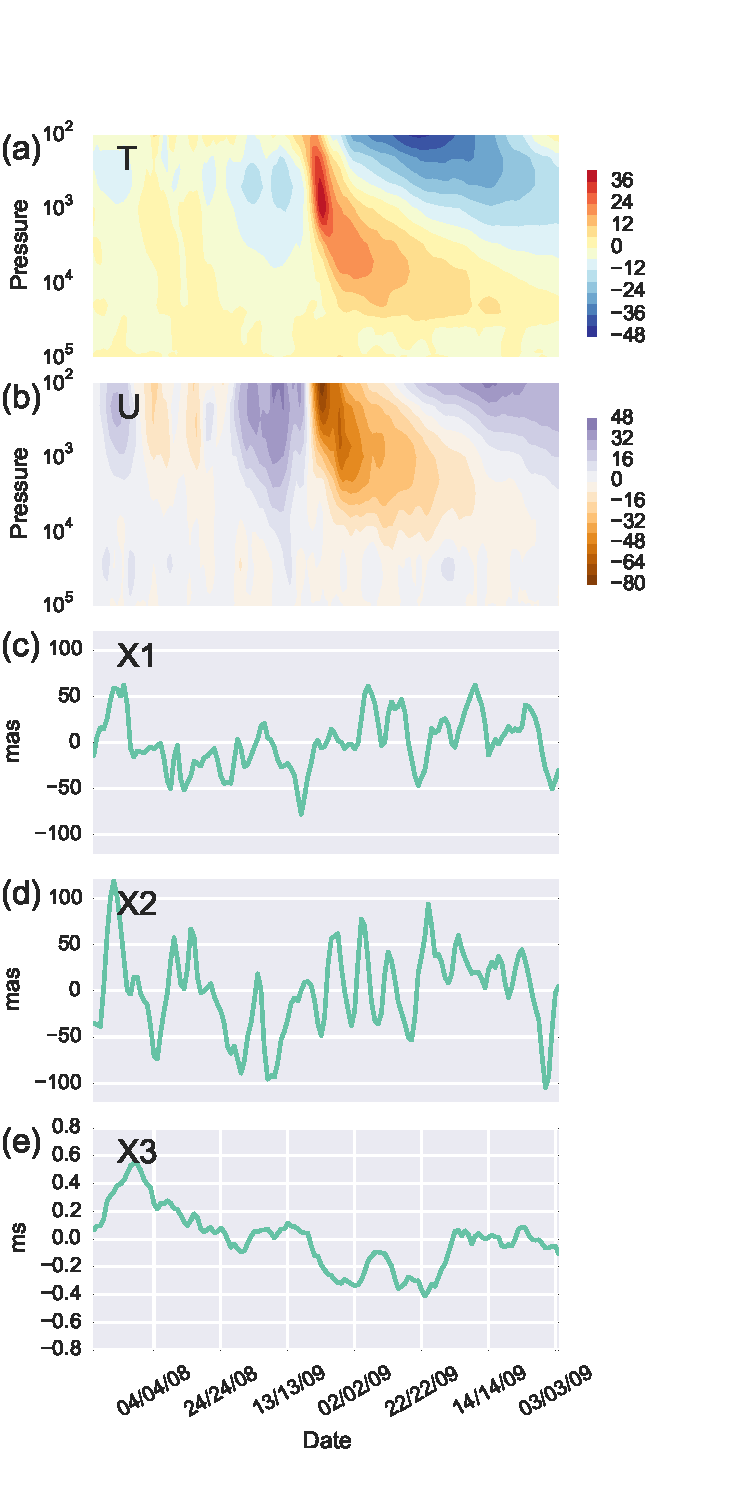
\includegraphics[width=0.5\textwidth]{Fig1.pdf} 
   \caption{First and second panels: altitude-time composites of the polar cap (60\degree-90\degree N) temperature and 60 \degree N zonal wind anomlies, for the January 2009 SSW event.  Bottom three panels: the observed anomalies in the three Earth rotation parameters over the same time. }  
   \label{fig:2009event}
 \end{figure}


\begin{figure} 
%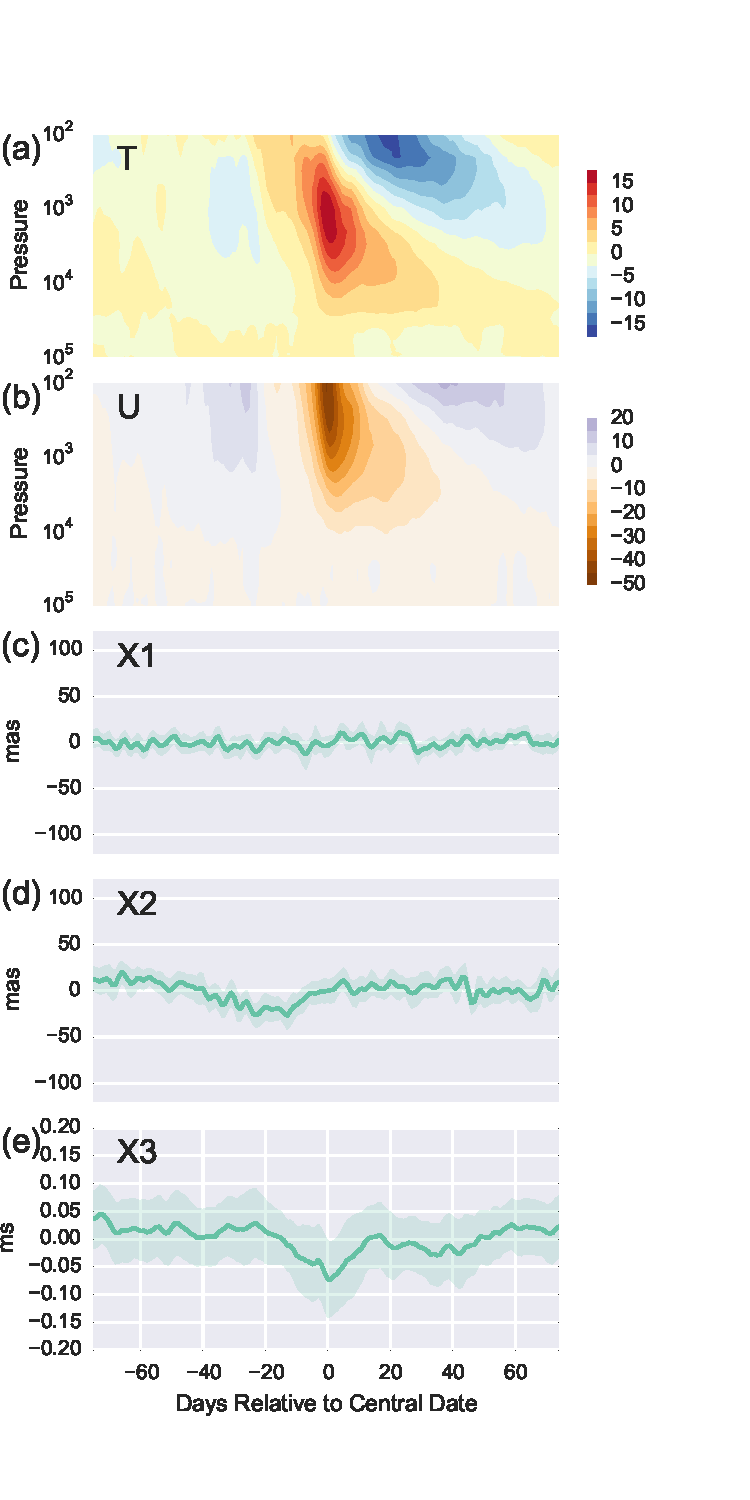
\includegraphics[width=0.5\textwidth]{Fig2.pdf}
   \caption{First and second panels: altitude-time composites of the polar cap (60\degree-90\degree N) temperature and 60 \degree N zonal wind anomlies, composited over the SSW events given in Table \ref{tab:warmings} and centered on the central date.  Bottom three panels: the observed anomalies in the three Earth rotation parameters composited over the same events.  The shading in ERP composites indicates the 96$\%$ bootstrap confidence interval.}
   \label{fig:summary}
 \end{figure}

\begin{figure}
  \noindent
%  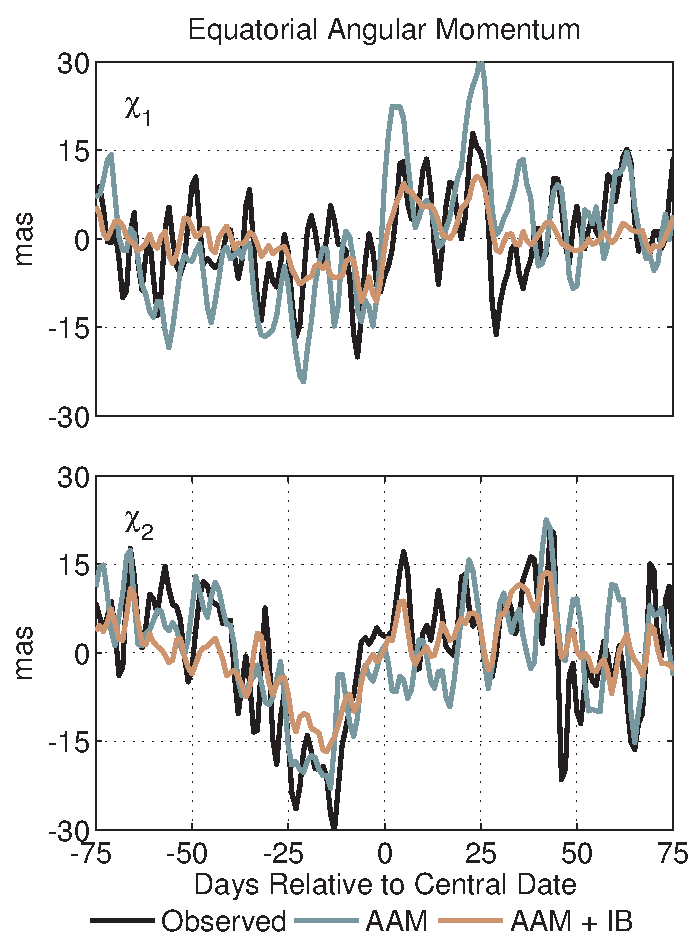
\includegraphics[width=0.8\textwidth]{Fig3.pdf} 
   \caption{Top: Composites of the $p_1$ anomaly (black) and the corresponding AAM mass excitation function  ($\chi_1^{\text{M}}$), with and without the IB approximation (see text), composited over  {the 22 major warming events in ERA-Interim}.   Bottom: As for top row but for observed $p_2$ anomaly and corresponding components of the mass excitation function $\chi_2^{\text{M}}$.}
   \label{fig:composites_X12}
 \end{figure}


\begin{figure}
  \noindent
% 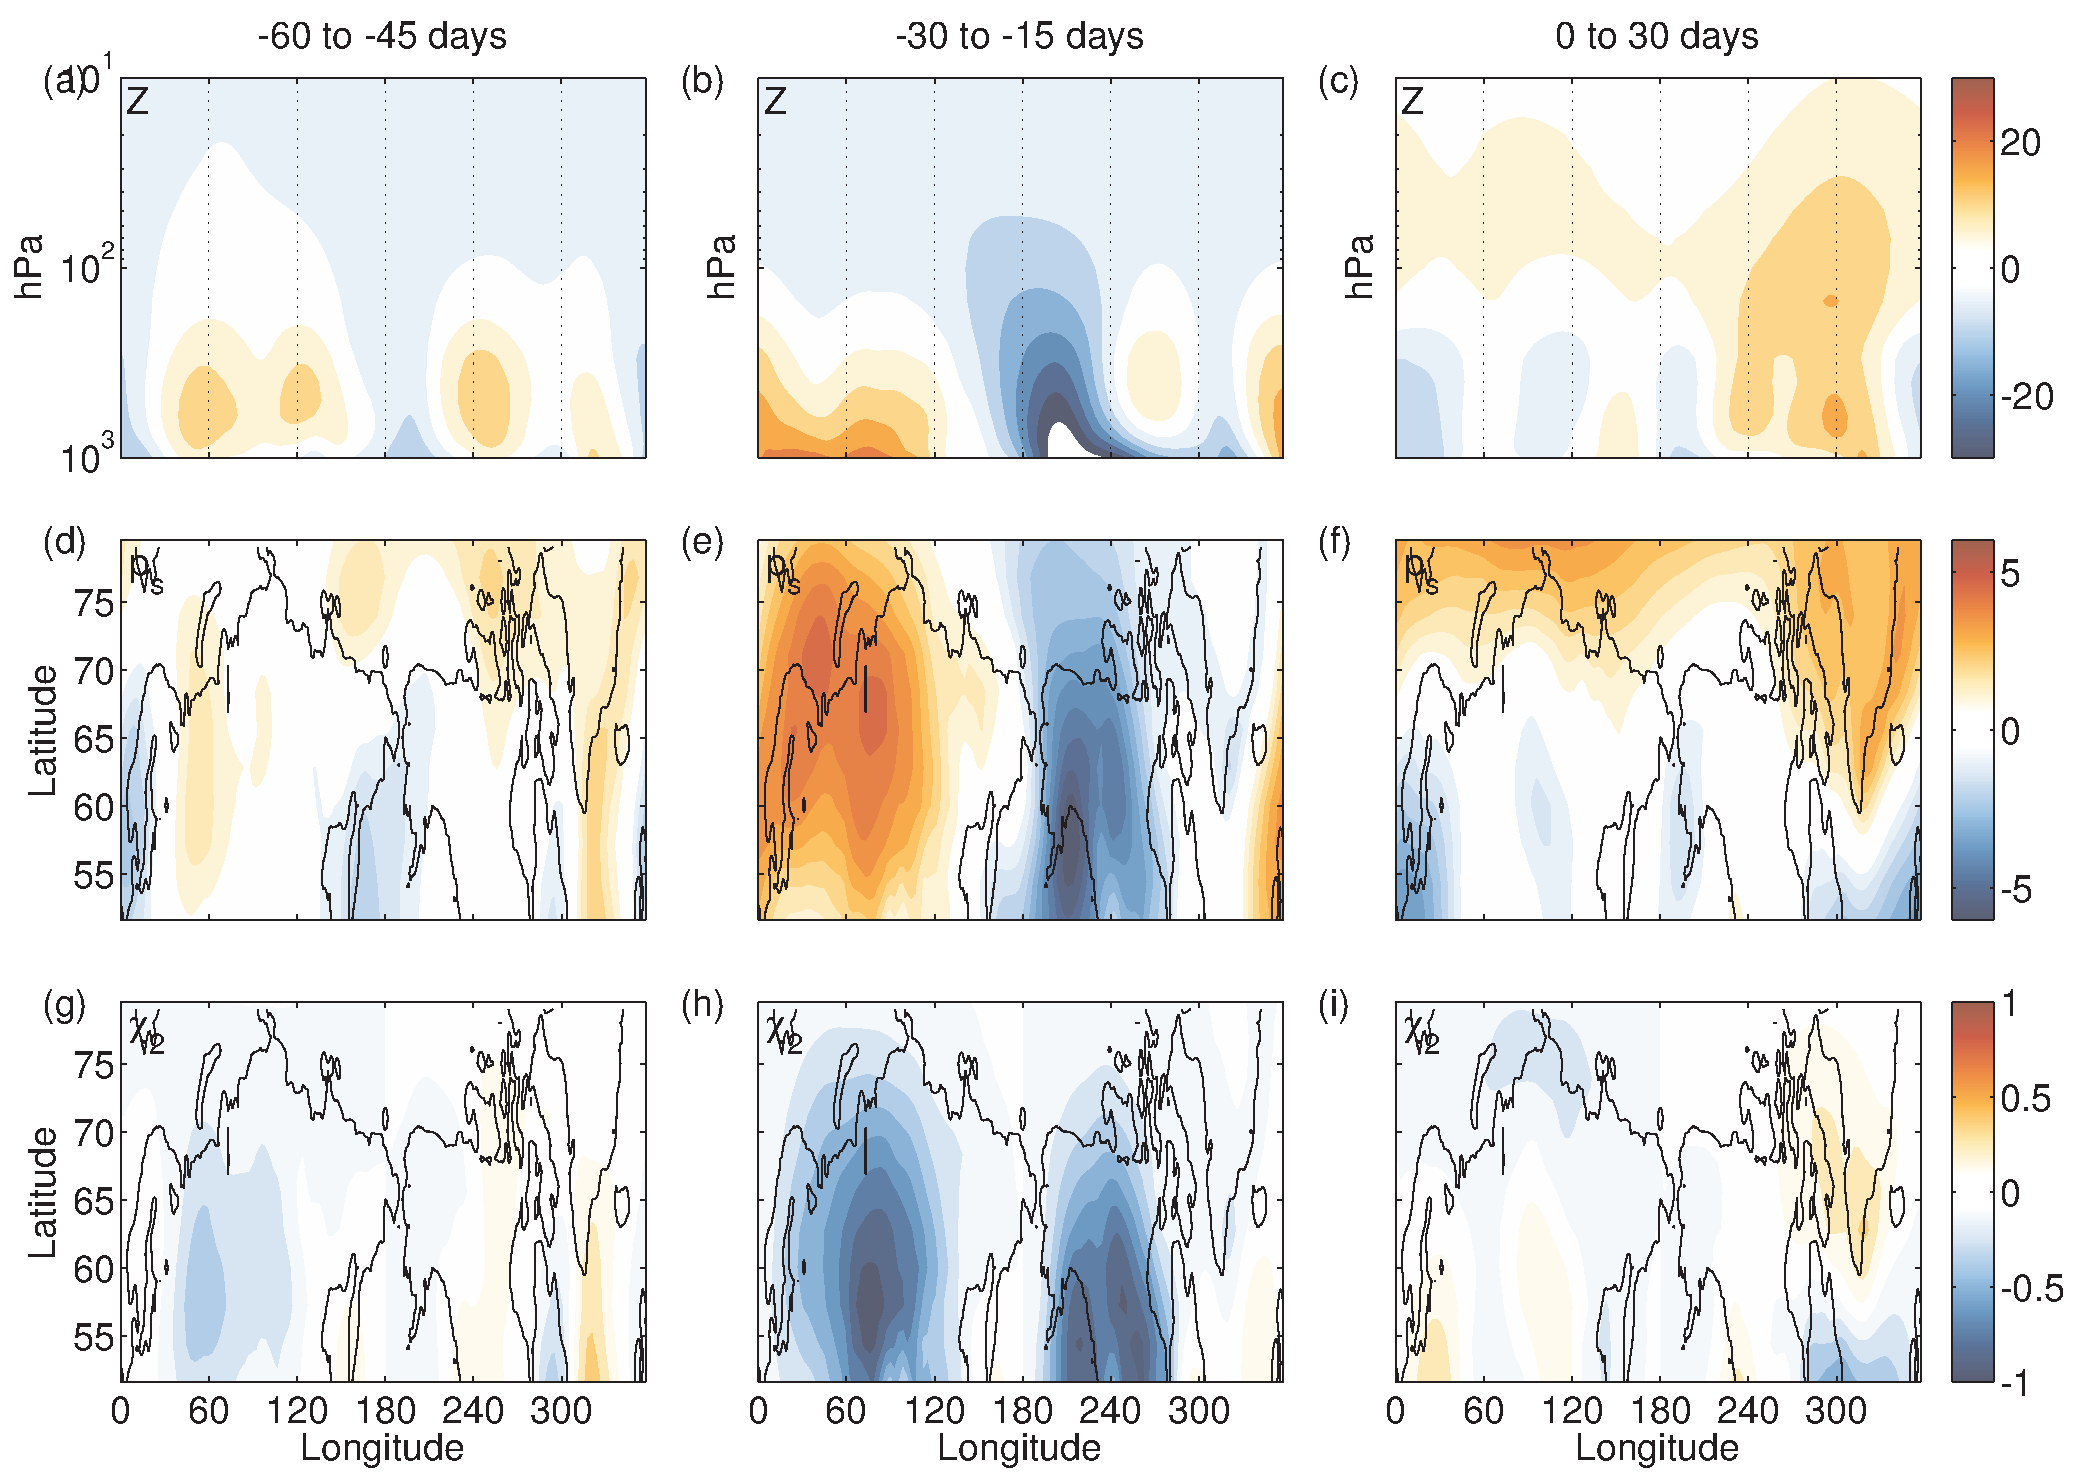
\includegraphics[width = \textwidth]{Fig4.pdf}
   \caption{Top row: Height-longitude cross sections of the geopotential height, composited over  {the 22 major warming events in ERA-Interim},  averaged over 3 periods before and after the central date.  Second row: the corresponding composite surface pressure anomaly.   {Bottom row}: the surface pressure anomalies weighted by  $\sin \phi \cos^2 \phi \sin \lambda$, as in the $\chi_2^{\text{M}}$ integral (eq. \ref{eq:X2m}).
}
   \label{fig:EGPH_mass_aam}
 \end{figure}

 
\begin{figure}
  \noindent
%  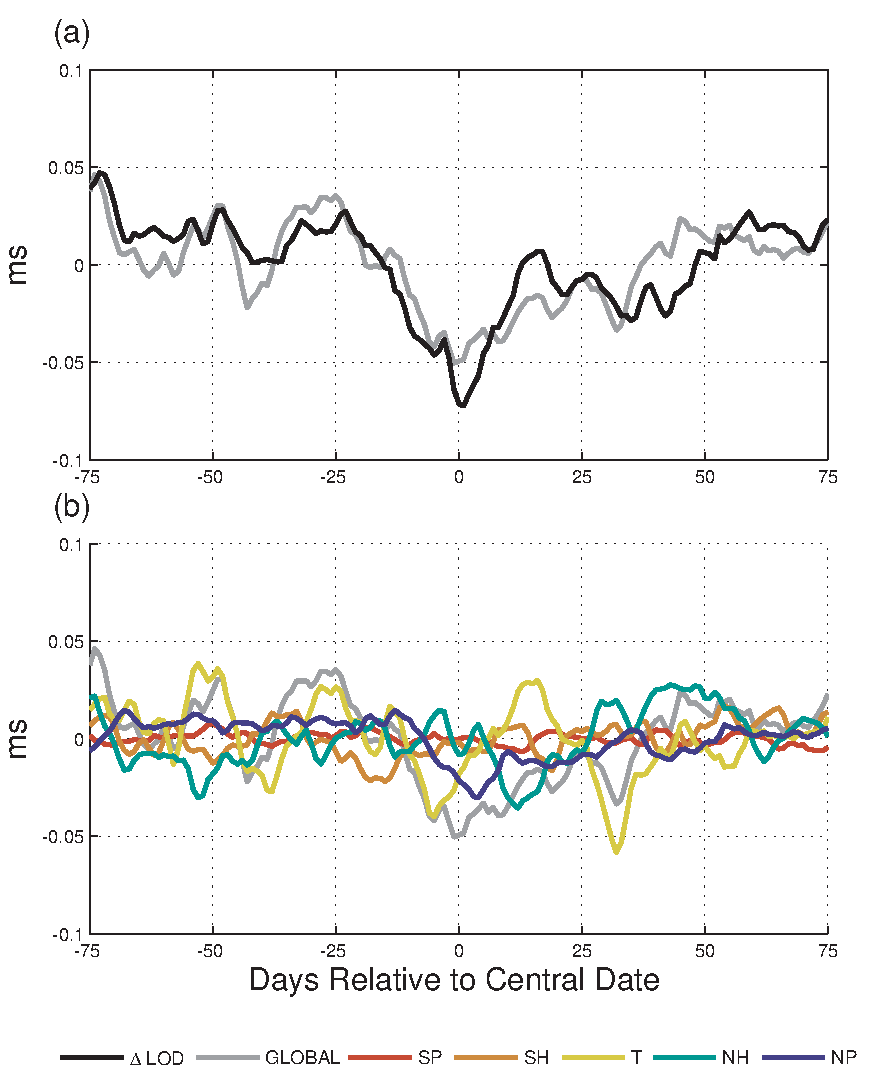
\includegraphics[width=0.7\textwidth]{Fig5.pdf} 
   \caption{ (a) the observed $\Delta$LOD (black) and the corresponding axial wind excitation ($\chi_3$, gray), composited over  {the all major warming events in the joint dataset} . (b): The composite wind excitation functions integrated over different latitude bands, along with the global value (gray). }
   \label{fig:composites_X3}
 \end{figure}

\begin{figure}
  \noindent
%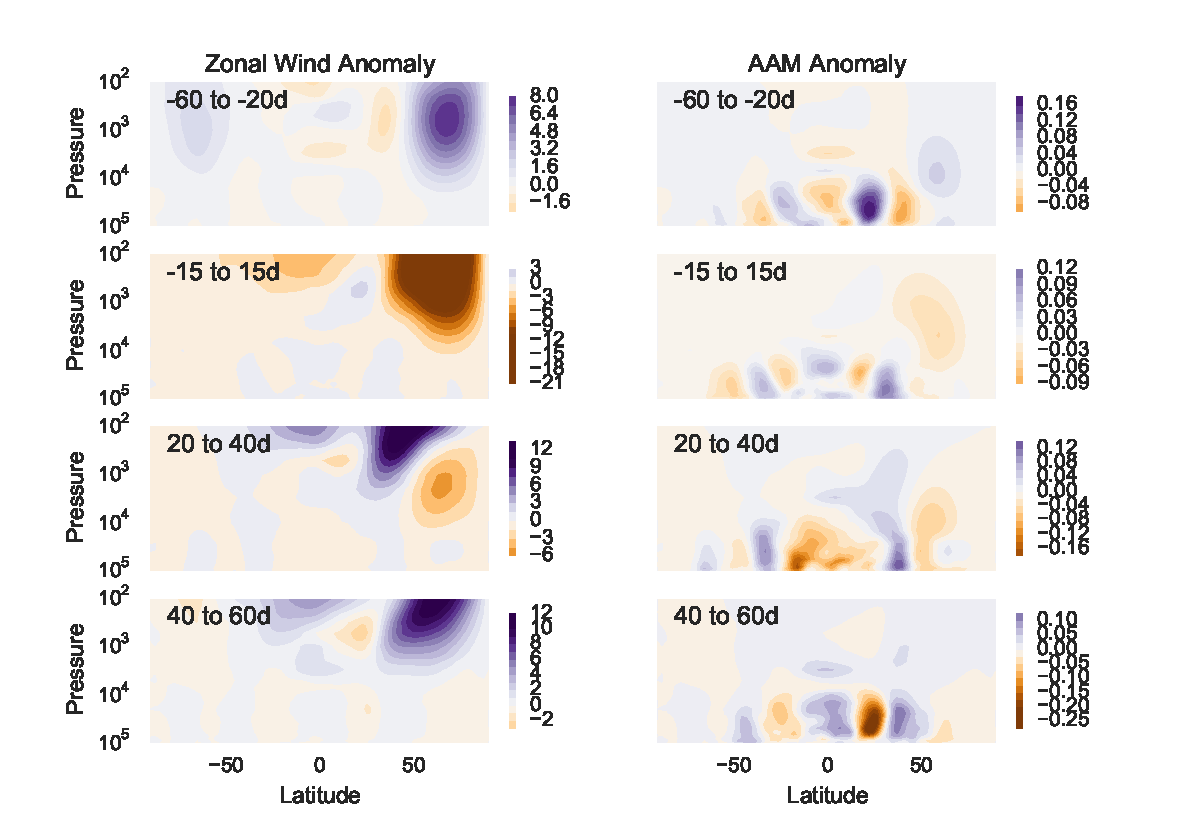
\includegraphics[width=\textwidth]{Fig6.pdf}
   \caption{ Left: Pressure-latitude slices of zonal-mean zonal wind, averaged over four blocks of time around the central date (see text), and composited over all SSW events in the joint dataset.  Right: multiplying the wind anomalies by $\cos^2 \phi$ and by the relative mass of each pressure level, such that each gridbox gives the local contribution to the global $\chi_3$ integral.
}
   \label{fig:wind_anomaly_composites}
 \end{figure}



\begin{figure}
  \noindent
%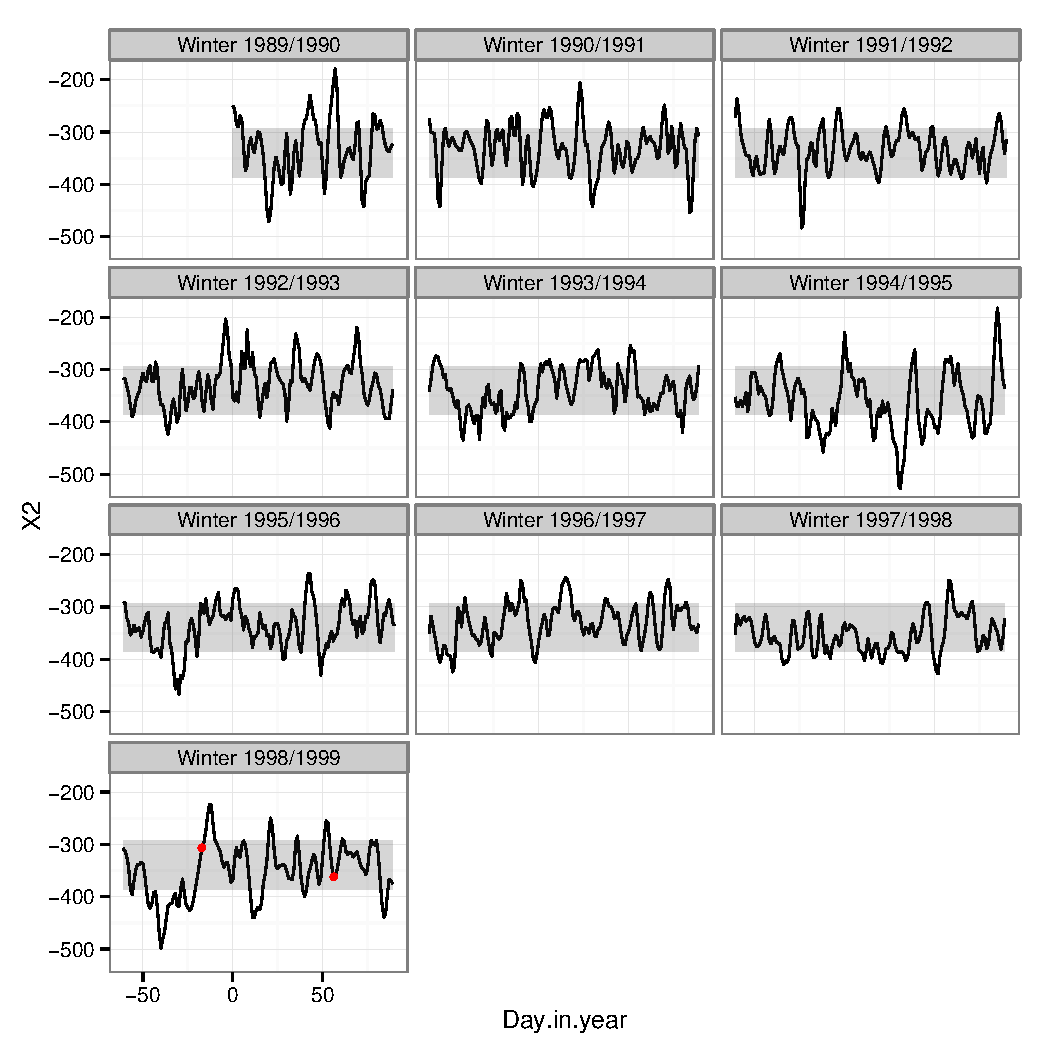
\includegraphics[width=\textwidth]{Fig7.pdf}
   \caption{$\chi_2^{\text{GEO}}$ for all 10 winters in the 1990s.  The mean and standard deviation of $\chi_2^{\text{GEO}}$ over the period 1962-2010 are shown by the shaded band in each plot, and the central dates of the  SSW events during this decade are shown by red dots.}
   \label{fig:X2_1990s}
 \end{figure}


\begin{figure}
  \noindent
%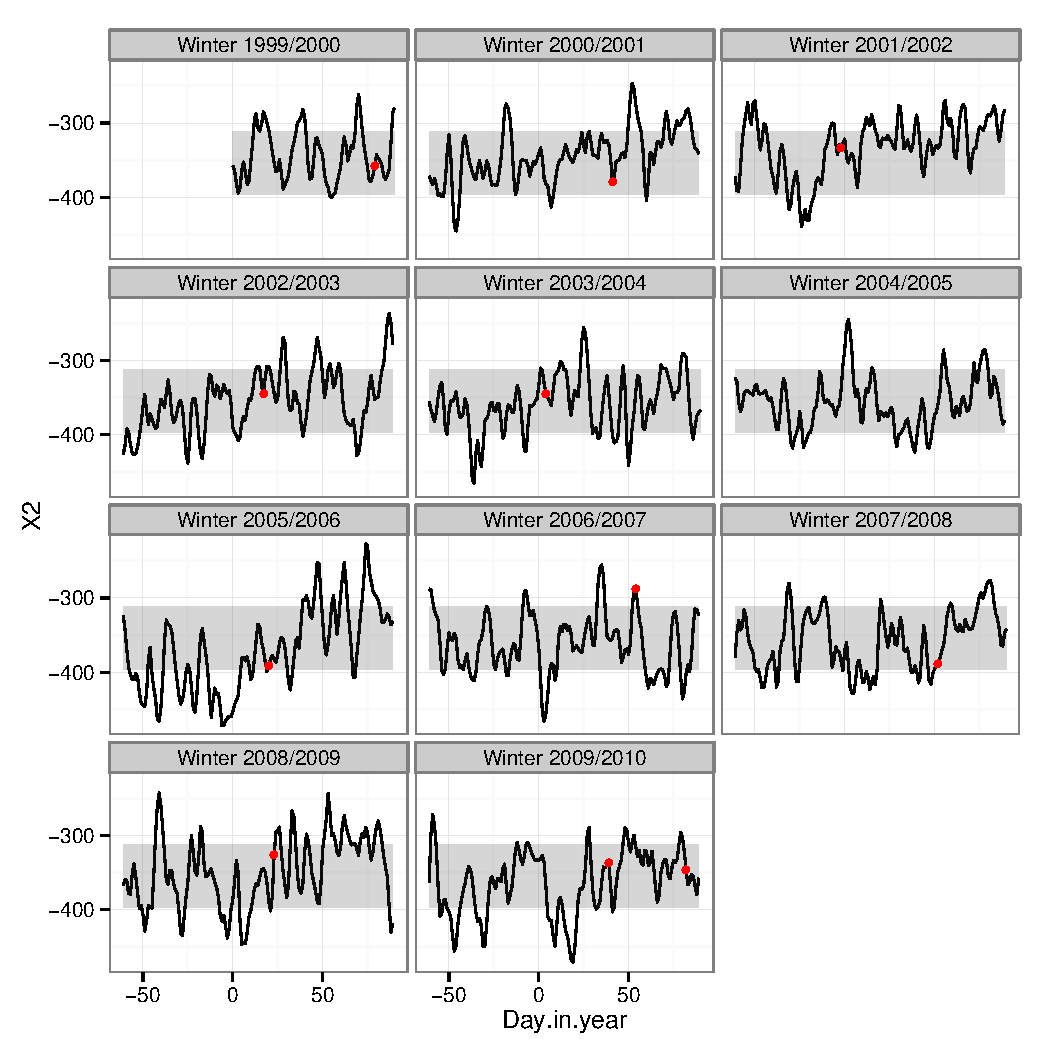
\includegraphics[width=\textwidth]{Fig8.pdf}
   \caption{As in Fig. \ref{fig:X2_1990s}, but for the first decade of the 2000s.  }
   \label{fig:X2_2000s}
 \end{figure}



% When submitting articles through the GEMS system:
% COMMENT OUT ANY COMMANDS THAT INCLUDE GRAPHICS.
%
% FOR FIGURES, DO NOT USE \psfrag or \subfigure commands.
%
% Figure captions go below the figure.
% Table titles go above tables; all other caption information
%  should be placed in footnotes below the table.

% DRAFT figure/table, including eps graphics
%
% \begin{figure}
% \noindent\includegraphics[width=20pc]{samplefigure.eps}
% \caption{Caption text here}
% \end{figure}
% \end{document}
%
% \begin{table}
% \caption{}
% \end{table}
%
% ---------------
% TWO-COLUMN figure/table
%
% \begin{figure*}
% \noindent\includegraphics[width=39pc]{samplefigure.eps}
% \caption{Caption text here}
% \end{figure*}
%
% \begin{table*}
% \caption{Caption text here}
% \end{table*}
%
% ---------------


% See below for how to make landscape/sideways figures or tables.

\end{document}

%%%%%%%%%%%%%%%%%%%%%%%%%%%%%%%%%%%%%%%%%%%%%%%%%%%%%%%%%%%%%%%

More Information and Advice:

%% ------------------------------------------------------------------------ %%
%
%  SECTION HEADS
%
%% ------------------------------------------------------------------------ %%

% Capitalize the first letter of each word (except for
% prepositions, conjunctions, and articles that are
% three or fewer letters).

% AGU follows standard outline style; therefore, there cannot be a section 1 without
% a section 2, or a section 2.3.1 without a section 2.3.2.
% Please make sure your section numbers are balanced.
% ---------------
% Level 1 head
%
% Use the \section{} command to identify level 1 heads;
% type the appropriate head wording between the curly
% brackets, as shown below.
%
%An example:
%\section{Level 1 Head: Introduction}
%
% ---------------
% Level 2 head
%
% Use the \subsection{} command to identify level 2 heads.
%An example:
%\subsection{Level 2 Head}
%
% ---------------
% Level 3 head
%
% Use the \subsubsection{} command to identify level 3 heads
%An example:
%\subsubsection{Level 3 Head}
%
%---------------
% Level 4 head
%
% Use the \subsubsubsection{} command to identify level 3 heads
% An example:
%\subsubsubsection{Level 4 Head} An example.
%
%% ------------------------------------------------------------------------ %%
%
%  IN-TEXT LISTS
%
%% ------------------------------------------------------------------------ %%
%
% Do not use bulleted lists; enumerated lists are okay.
% \begin{enumerate}
% \item
% \item
% \item
% \end{enumerate}
%
%% ------------------------------------------------------------------------ %%
%
%  EQUATIONS
%
%% ------------------------------------------------------------------------ %%

% Single-line equations are centered.
% Equation arrays will appear left-aligned.

Math coded inside display math mode \[ ...\]
 will not be numbered, e.g.,:
 \[ x^2=y^2 + z^2\]

 Math coded inside \begin{equation} and \end{equation} will
 be automatically numbered, e.g.,:
 \begin{equation}
 x^2=y^2 + z^2
 \end{equation}

% IF YOU HAVE MULTI-LINE EQUATIONS, PLEASE
% BREAK THE EQUATIONS INTO TWO OR MORE LINES
% OF SINGLE COLUMN WIDTH (20 pc, 8.3 cm)
% using double backslashes (\\).

% To create multiline equations, use the
% \begin{eqnarray} and \end{eqnarray} environment
% as demonstrated below.
\begin{eqnarray}
  x_{1} & = & (x - x_{0}) \cos \Theta \nonumber \\
        && + (y - y_{0}) \sin \Theta  \nonumber \\
  y_{1} & = & -(x - x_{0}) \sin \Theta \nonumber \\
        && + (y - y_{0}) \cos \Theta.
\end{eqnarray}

%If you don't want an equation number, use the star form:
%\begin{eqnarray*}...\end{eqnarray*}

% Break each line at a sign of operation
% (+, -, etc.) if possible, with the sign of operation
% on the new line.

% Indent second and subsequent lines to align with
% the first character following the equal sign on the
% first line.

% Use an \hspace{} command to insert horizontal space
% into your equation if necessary. Place an appropriate
% unit of measure between the curly braces, e.g.
% \hspace{1in}; you may have to experiment to achieve
% the correct amount of space.


%% ------------------------------------------------------------------------ %%
%
%  EQUATION NUMBERING: COUNTER
%
%% ------------------------------------------------------------------------ %%

% You may change equation numbering by resetting
% the equation counter or by explicitly numbering
% an equation.

% To explicitly number an equation, type \eqnum{}
% (with the desired number between the brackets)
% after the \begin{equation} or \begin{eqnarray}
% command.  The \eqnum{} command will affect only
% the equation it appears with; LaTeX will number
% any equations appearing later in the manuscript
% according to the equation counter.
%

% If you have a multiline equation that needs only
% one equation number, use a \nonumber command in
% front of the double backslashes (\\) as shown in
% the multiline equation above.

%% ------------------------------------------------------------------------ %%
%
%  LANDSCAPE/SIDEWAYS FIGURE AND TABLE EXAMPLES
%
%% ------------------------------------------------------------------------ %%
%
% For figures, add \usepackage{lscape} to the file and the landscape.sty style file
% to the paper folder.
%
% \begin{figure*}[p]
% \begin{landscapefigure*}
% Illustration here.
% \caption{caption here}
% \end{landscapefigure*}
% \end{figure*}
%
% For tables, add \usepackage{rotating} to the paper and add the rotating.sty file to the folder.
%
% AGU prefers the use of {sidewaystable} over {landscapetable} as it causes fewer problems.
%
% \begin{sidewaystable}
% \caption{}
% \begin{tabular}
% Table layout here.
% \end{tabular}
% \end{sidewaystable}
%
%

